\documentclass[10pt]{beamer}

\usetheme{metropolis}
\usepackage{appendixnumberbeamer}

\usepackage{booktabs}
\usepackage[scale=2]{ccicons}

\usepackage{pgfplots}
\usepgfplotslibrary{dateplot}

\usepackage{graphicx}
\graphicspath{ {imgs/} }

\usepackage{subcaption}

\usepackage{hyperref}

\usepackage{xspace}
\newcommand{\themename}{\textbf{\textsc{metropolis}}\xspace}

\title{Introduction to Deep Learning}
%\subtitle{A modern beamer theme}
\date{\today}
\author{Paul Drăgan}
\institute{Research in Cluj}
% \titlegraphic{\hfill\includegraphics[height=1.5cm]{logo.pdf}}

\begin{document}

\maketitle
%
%\begin{frame}{Table of contents}
%  \setbeamertemplate{section in toc}[sections numbered]
%  \tableofcontents[hideallsubsections]
%\end{frame}

\section{Machine Learning}

\begin{frame}{What is machine learning?}
	\begin{columns}
		\begin{column}{0.4\textwidth}
			\onslide<2->{
			To \alert{learn} $=$ algorithmically find the choice of parameters that best explain the data.}
		\end{column}
		\begin{column}{0.6\textwidth}
			\onslide<3->{
			\begin{exampleblock}{Example learning tasks}
				Find the line that best fits the points. Find giraffes in pictures.
			\end{exampleblock}
			\begin{center}
			\begin{figure}
			    \centering
			    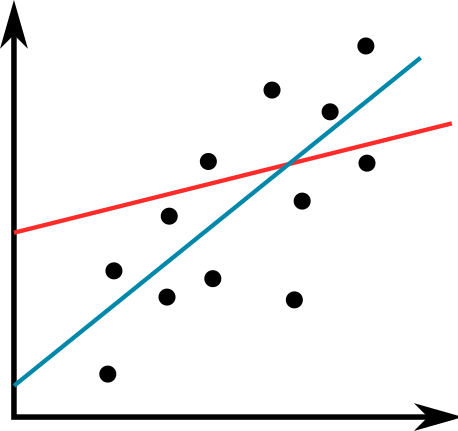
\includegraphics[width=0.4\linewidth]{intro_ml_1}
		    \end{figure}
		    \begin{figure}
		    	\centering
		    	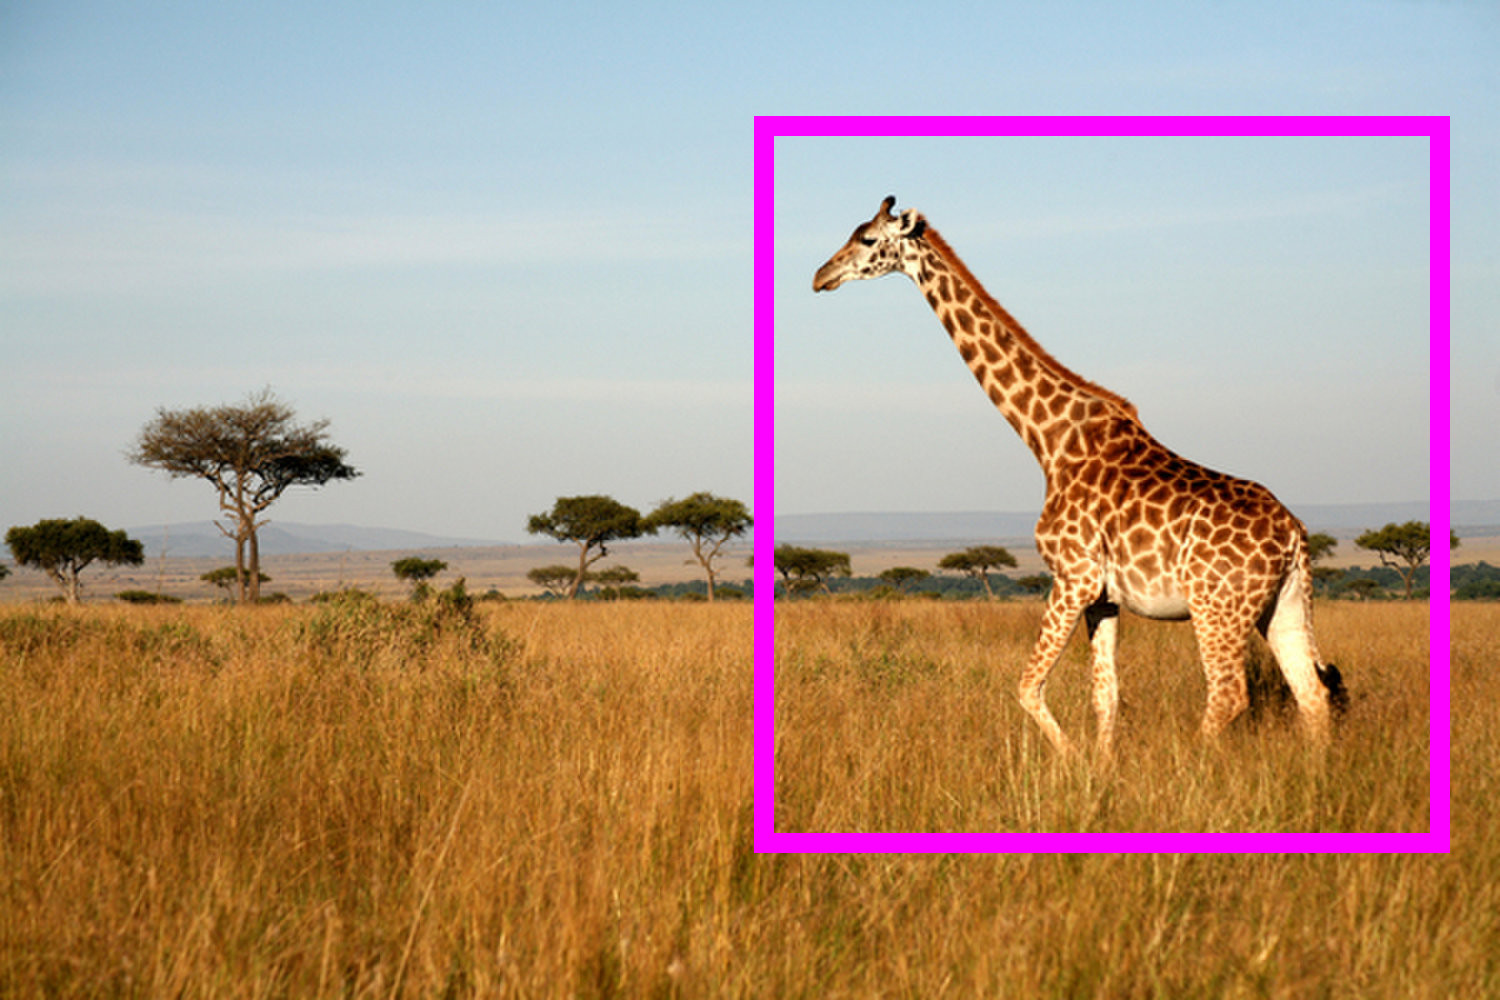
\includegraphics[scale=0.4]{giraffe1_detected}
		    \end{figure}}
		    \end{center}
		\end{column}
	\end{columns}
\end{frame}

\begin{frame}{Machine learning - Where are we now?}
	Current uses of ML algorithms in industry:
	\begin{itemize}
		\item<2-> speech recognition
		\item<3-> image classification
		\item<4-> object recognition
		\item<5-> spam filters and fraud detection
		\item<6-> automatic email labeling and sorting
		\item<7-> personalized search results and recommendations
		\item<8-> automatic image captioning
		\item<9-> online advertising
		\item<10-> medical diagnosis
		\item<11-> language understanding and translation
	\end{itemize}
\end{frame}

\begin{frame}{Machine learning - Where do we want to be?}
\begin{columns}
	\begin{column}{0.5\textwidth}
		\onslide<2->{In the short term:}
			\begin{itemize}
				\item<3-> increase robustness
				\item<4-> improve scalability 
				\item<5-> better testing procedures
				\item<6-> extend areas of application
				\item<7-> improve sample efficiency
			\end{itemize}
	\end{column}
	\begin{column}{0.5\textwidth}
		\onslide<8->{In the long term:}
			\begin{itemize}
				%\item more general algorithms
				\item<9-> algorithms that learn what to learn
				\item<10-> general AI?
			\end{itemize}
%		\begin{figure}
%			\begin{subfigure}{0.5\textwidth}
%				\centering
%				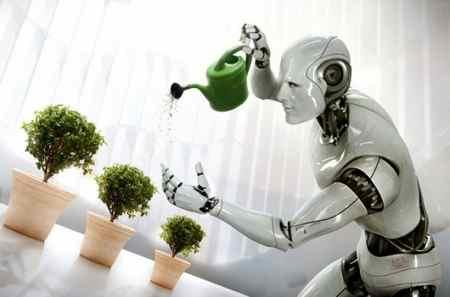
\includegraphics[width=\linewidth]{robot1}
%			\end{subfigure}%
%			\begin{subfigure}{0.5\textwidth}
%				\centering
%				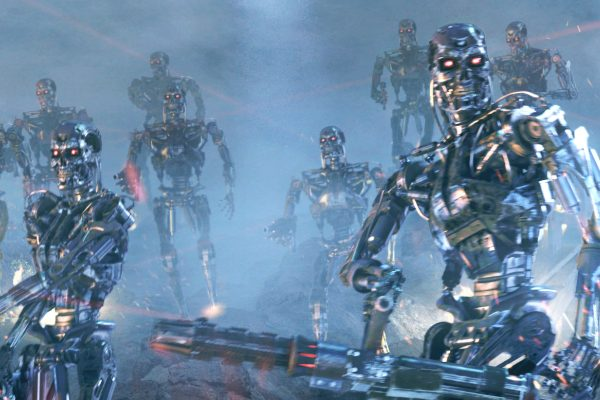
\includegraphics[width=\linewidth]{terminator}
%			\end{subfigure}
%		\end{figure}
		\onslide<10->{
		\begin{figure}
			\centering
			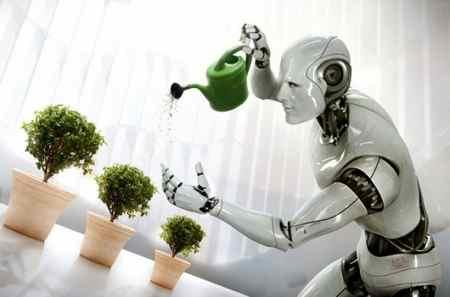
\includegraphics[width=0.6\linewidth]{robot1}
		\end{figure}
		\begin{figure}
			\centering
			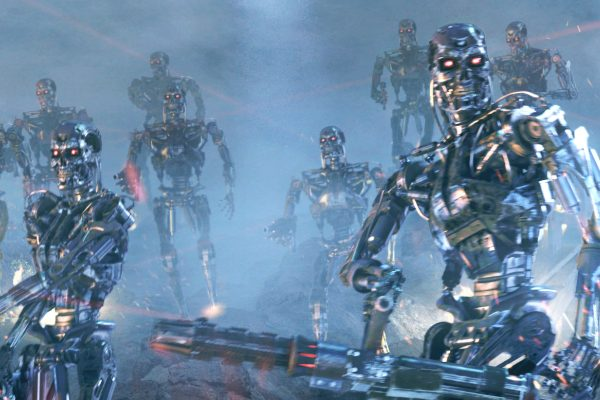
\includegraphics[width=0.6\linewidth]{terminator}
		\end{figure}}
	\end{column}
\end{columns}
\end{frame}

\begin{frame}{Machine learning - Common algorithms}
	\begin{columns}
		\begin{column}{0.5\textwidth}
			Commonly used algorithms are:
			\begin{itemize}
				\item<2-> K-means clustering
				\item<3-> Decision trees
				\item<4-> Support vector machines
				\item<5-> Bayesian networks
				\item<6-> \alert{Deep learning / Neural networks}
			\end{itemize}
		\end{column}
		\begin{column}{0.5\textwidth}
			\begin{figure}
				\begin{subfigure}{.5\textwidth}
					\centering
					\onslide<2->{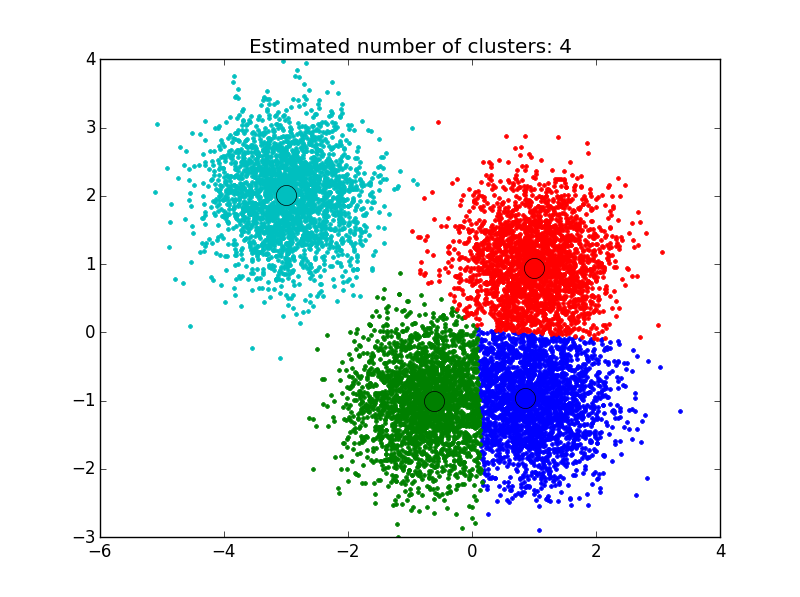
\includegraphics[width=\linewidth]{kmeans-clustering}}
				\end{subfigure}%
				\begin{subfigure}{.5\textwidth}
					\centering
					\onslide<3->{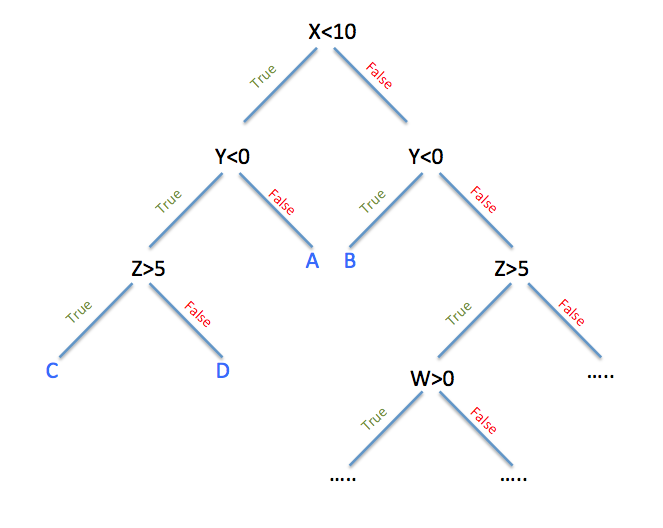
\includegraphics[width=\linewidth]{decisiontrees}}
				\end{subfigure}
				\begin{subfigure}{.5\textwidth}
					\centering
					\onslide<4->{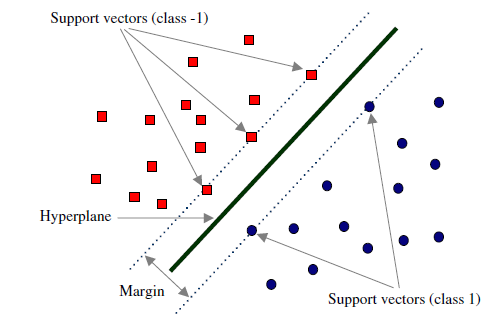
\includegraphics[width=\linewidth]{supportvectormachines}}
				\end{subfigure}%
				\begin{subfigure}{.5\textwidth}
					\centering
					\onslide<5->{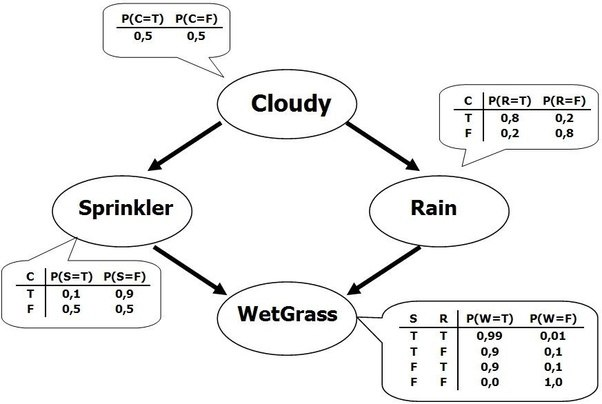
\includegraphics[width=\linewidth]{bayesian-networks}}
				\end{subfigure}
				\begin{subfigure}{\textwidth}
					\centering
					\onslide<6->{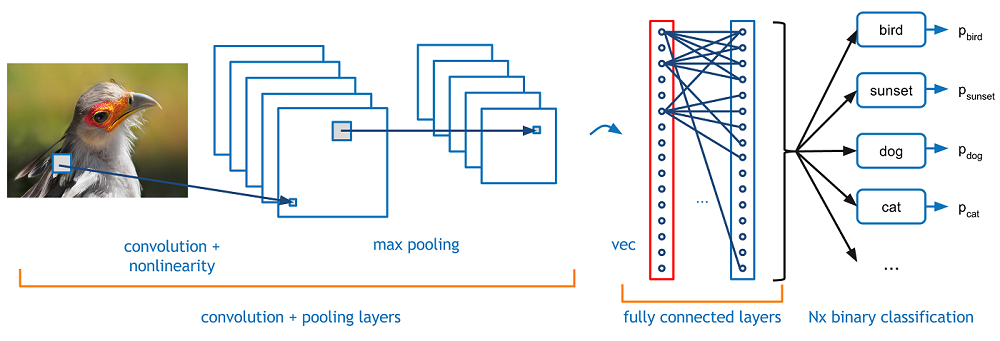
\includegraphics[width=\linewidth]{deeplearning-intro-ml}}
				\end{subfigure}		
			\end{figure}
		\end{column}
	\end{columns}
\end{frame}

\section{Deep learning}
\begin{frame}{Deep learning - What is it?}
	\onslide<2->{
	\begin{figure}
		\centering
		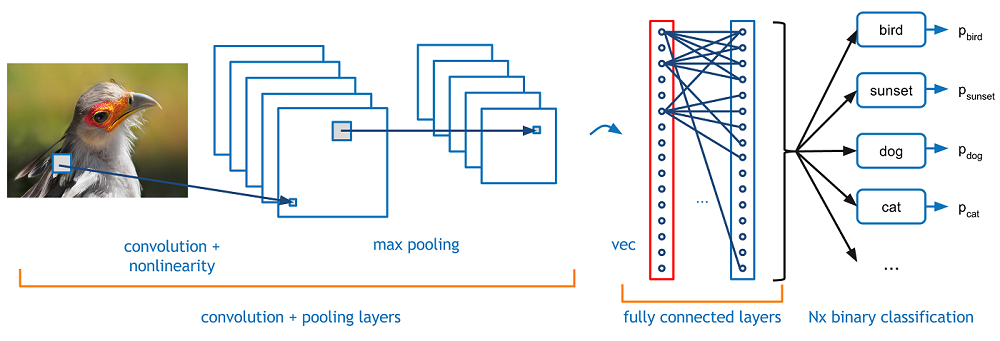
\includegraphics[width=\linewidth]{deeplearning-intro-ml}
		\caption{Arguably complicated figure that you won't understand.}
	\end{figure}}
	\onslide<3->{
	Deep learning:}
	\begin{itemize}
		\item<4-> A particular \alert{subset} of ML algorithms a.k.a. ``enhanced neural networks''
		\item<5-> The closest to an \alert{ideal learning agent}
	\end{itemize}
\end{frame}

\begin{frame}{Ideal learning agent}
	\only<1>{\begin{figure}
		\centering
		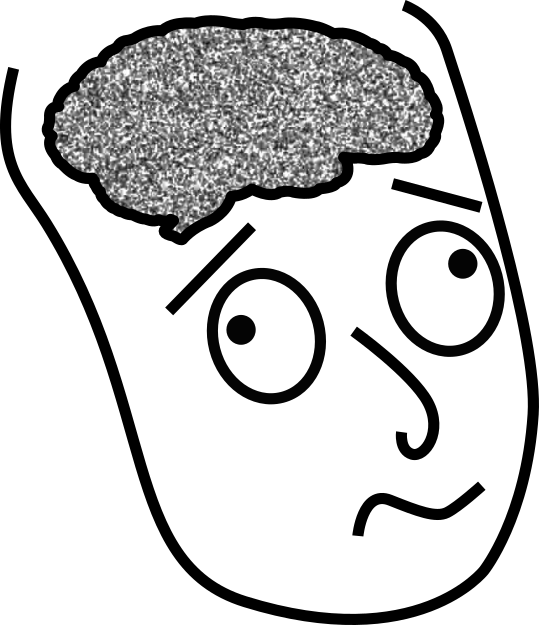
\includegraphics[scale=0.5]{getting_smart_1}
	\end{figure}}
	\only<2>{\begin{figure}
		\centering
		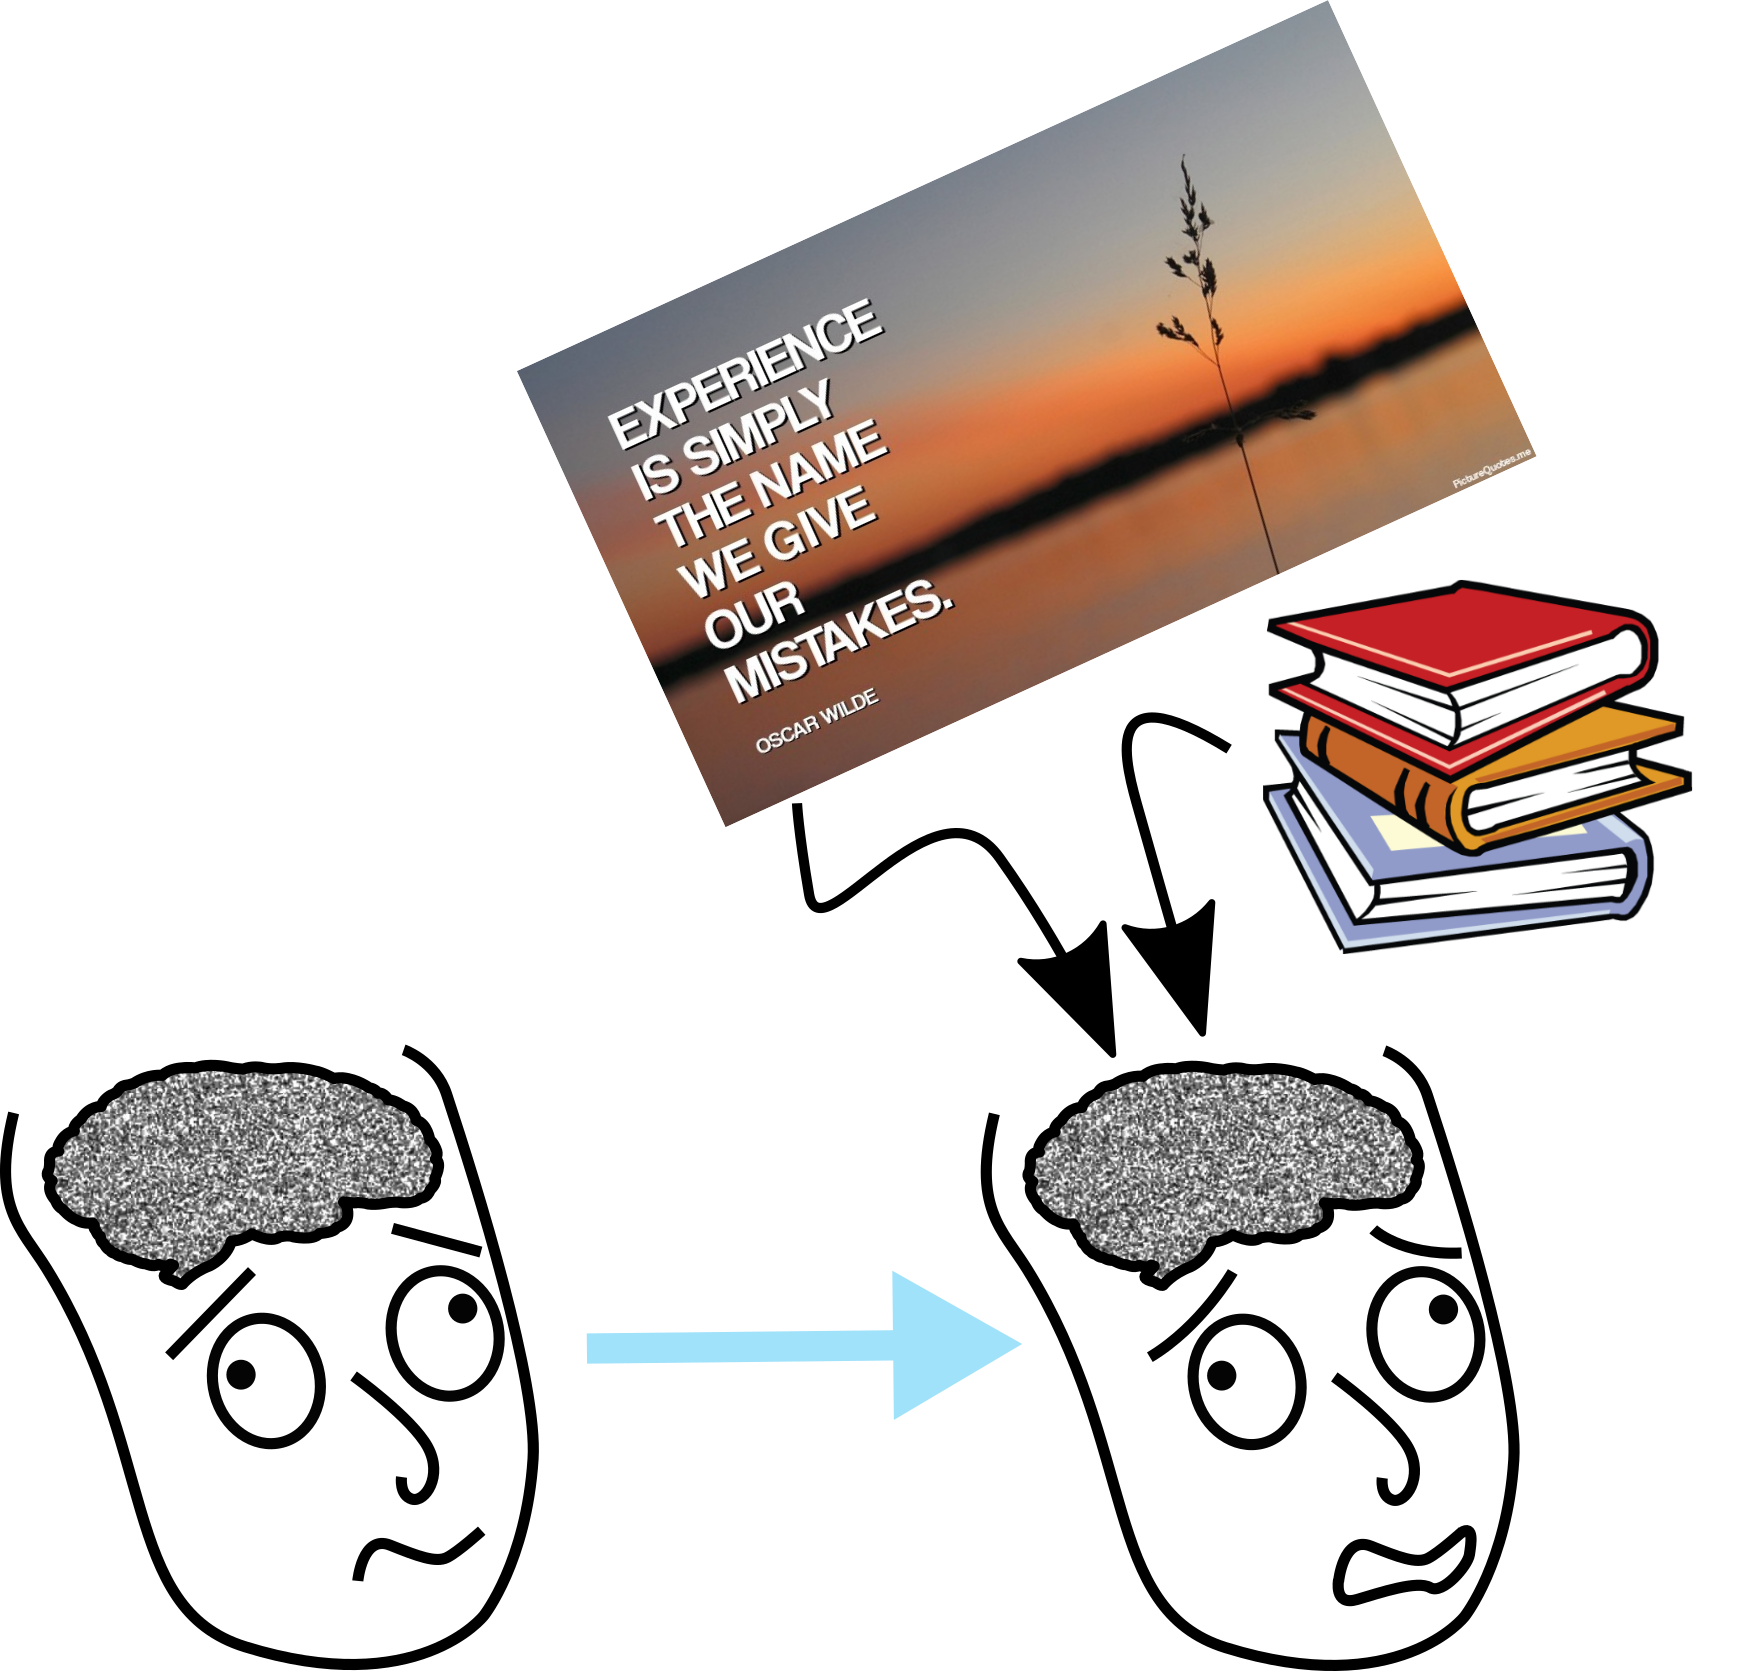
\includegraphics[scale=0.5]{getting_smart_2}
	\end{figure}}
	\only<3>{\begin{figure}
		\centering
		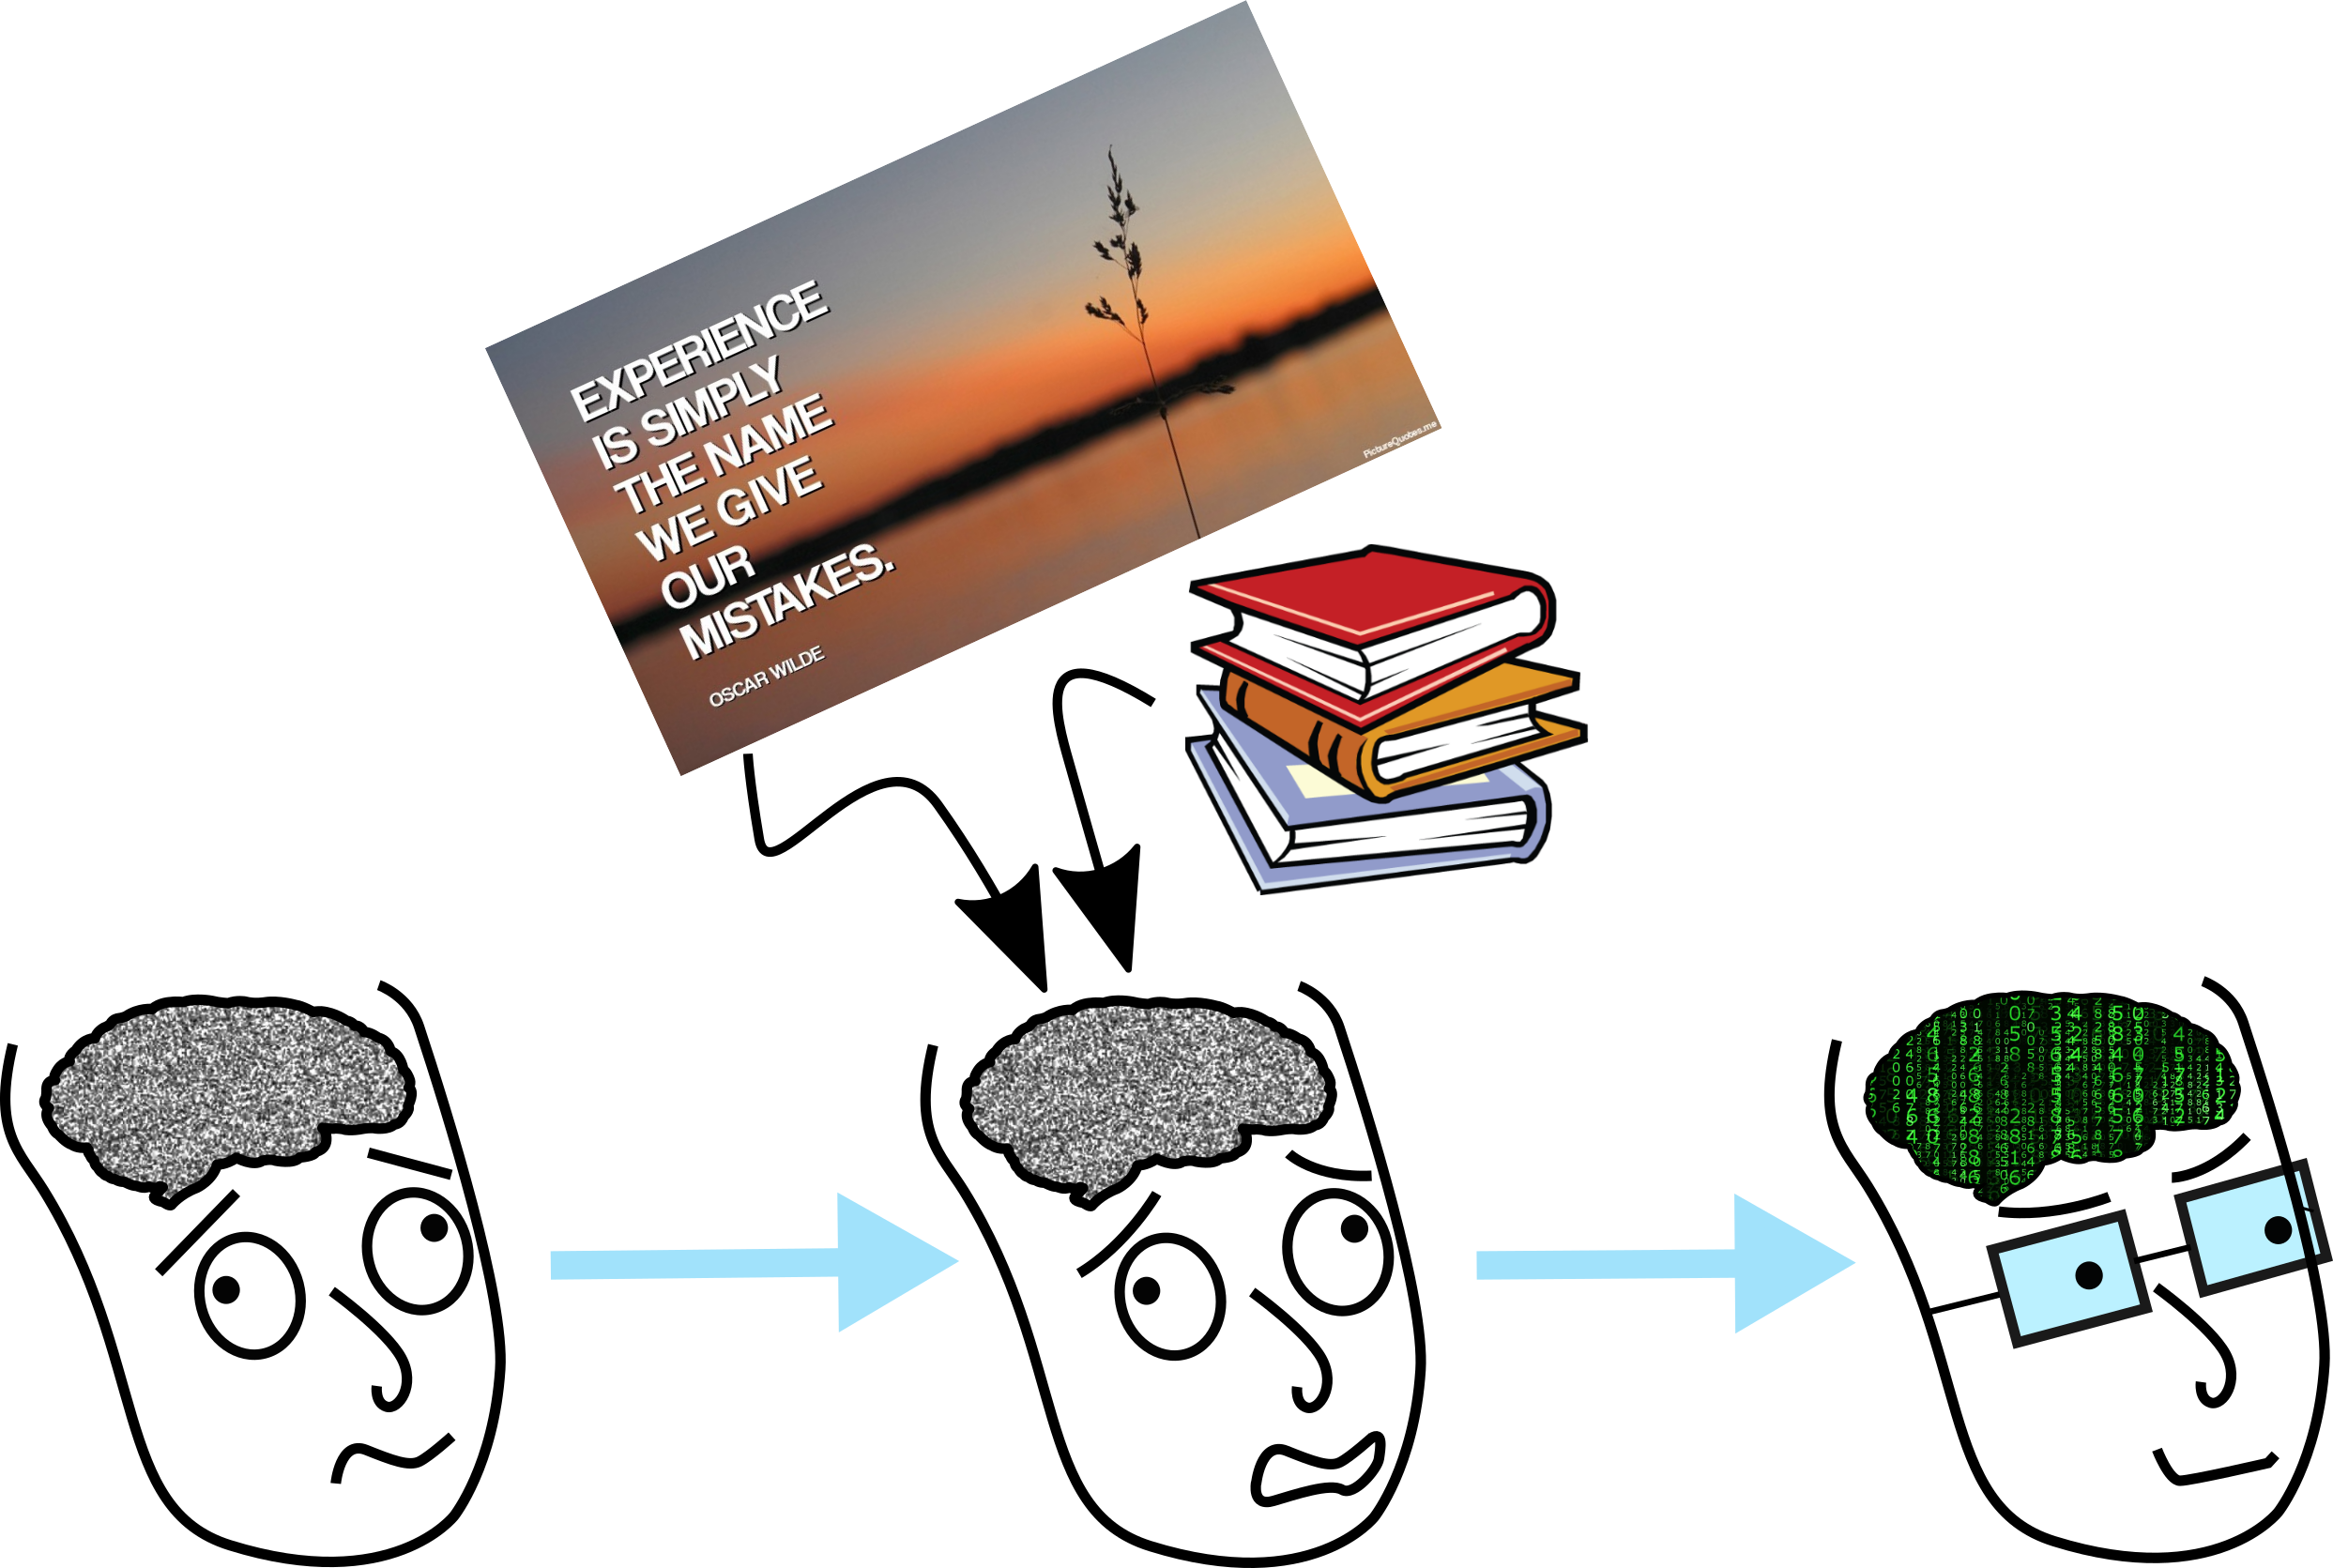
\includegraphics[scale=0.5]{getting_smart_3}
	\end{figure}}
\end{frame}

\begin{frame}{Enhanced neural networks}
	\onslide<2->{
	\begin{quote}
		``Deep learning'' can be translated to: ``enhanced neural networks''.
	\end{quote}
	\begin{flushright}
		-- Paul Drăgan, some minutes ago
	\end{flushright}}
\end{frame}

\begin{frame}{Artifical neuron}
	\begin{columns}
		\begin{column}{0.6\textwidth}
			\onslide<2->{
			\begin{figure}
				\centering
				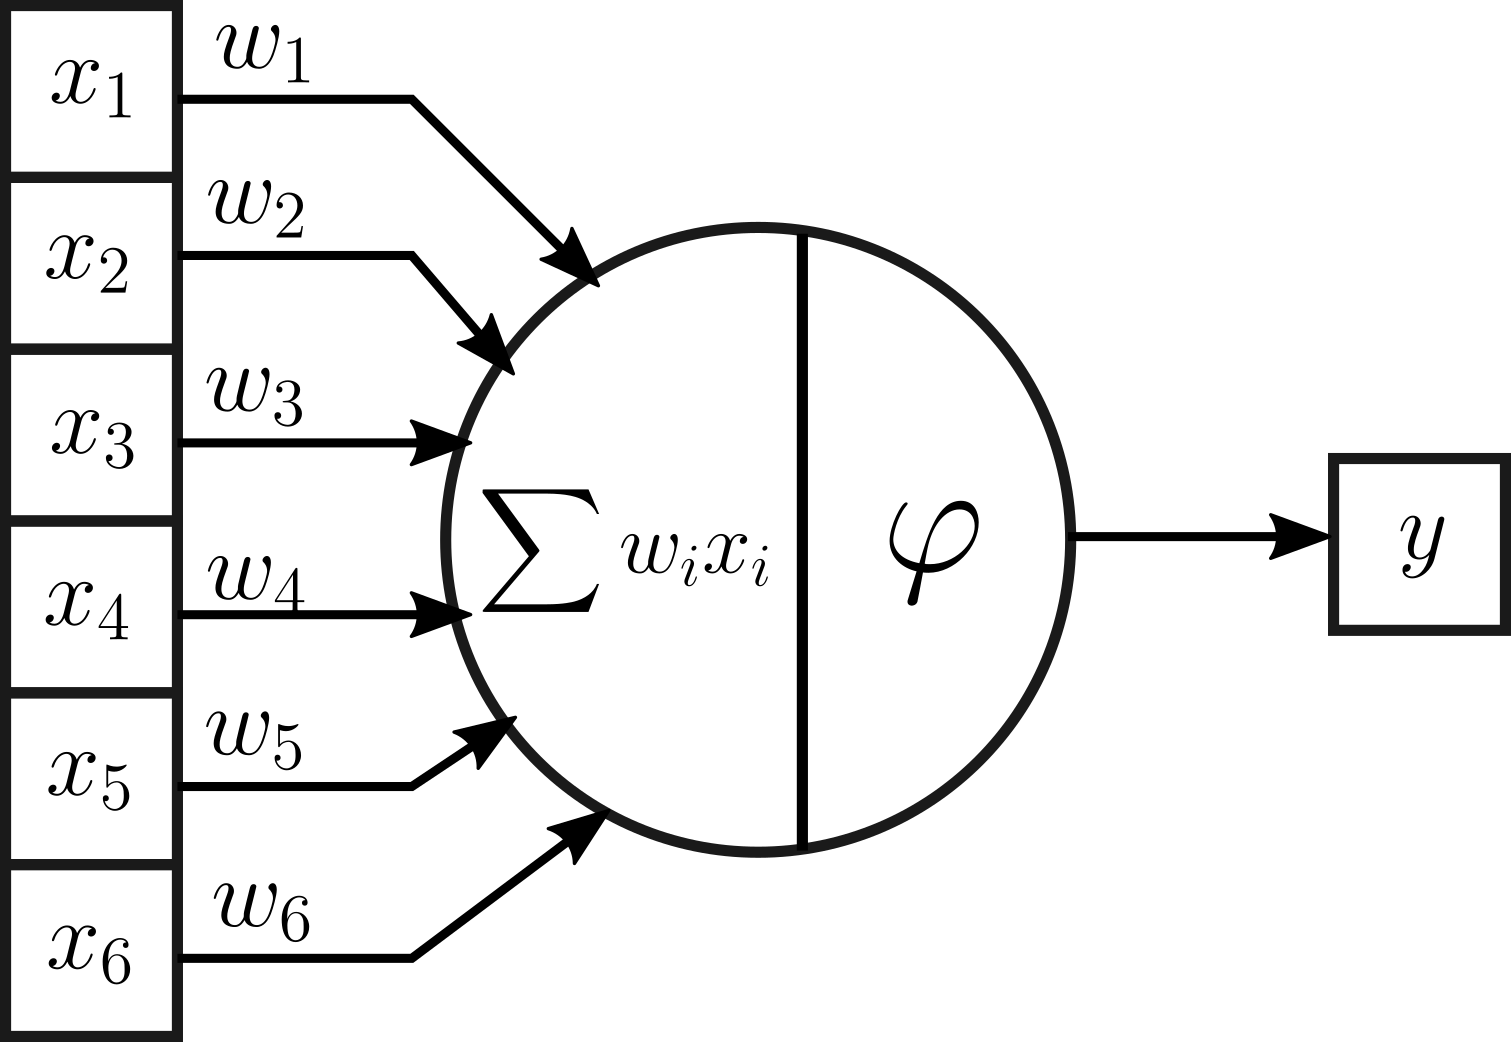
\includegraphics[width=0.8\linewidth]{artificial_neuron}
			\end{figure}}
			\onslide<4->{
			\begin{figure}
				\centering
				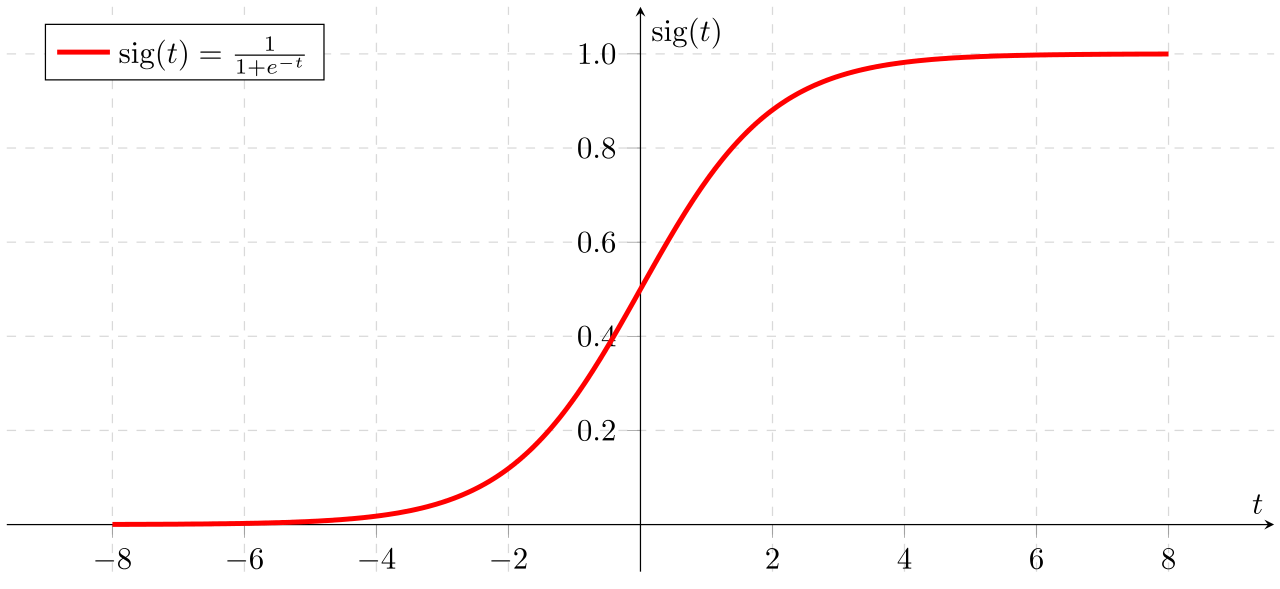
\includegraphics[width=0.7\linewidth]{sigmoid}
				\\{The sigmoid activation function $\varphi$.}
			\end{figure}}
		\end{column}
		\begin{column}{0.4\textwidth}
			\onslide<3->{
		    Where:
			\begin{itemize}
				\item $x_i$ are the inputs
				\item $w_i$ are the weights
				\item $\varphi$ is the activation function
				\item $y$ is the output
			\end{itemize}}
			\onslide<5->{
			The weights $w_i$ are \alert{free parameters} -> they can be \alert{trained} / \alert{learned}.}
		\end{column}
	\end{columns}
\end{frame}

\begin{frame}{Neural networks}
	\begin{figure}
		\centering
		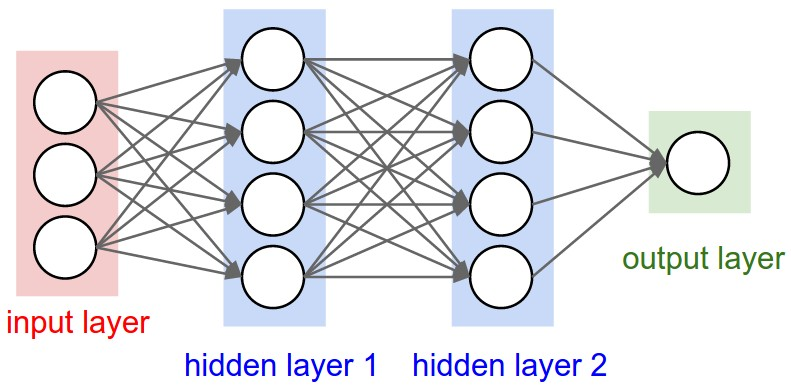
\includegraphics[width=0.8\linewidth]{neuralnetwork2}
	\end{figure}
	\onslide<2->{
	Neural networks are theoretically guaranteed to be \alert{universal function approximators}.}
\end{frame}

\begin{frame}{Universal function approximators}
	\onslide<2->{
	Simple mathematical functions:
	\begin{equation*}
		x \mapsto y \qquad  f(x) = x^2+1 = y
	\end{equation*}}
	\onslide<3->{
	Giraffe detection:
	\begin{figure}
		\begin{subfigure}{0.4\linewidth}
			\centering
			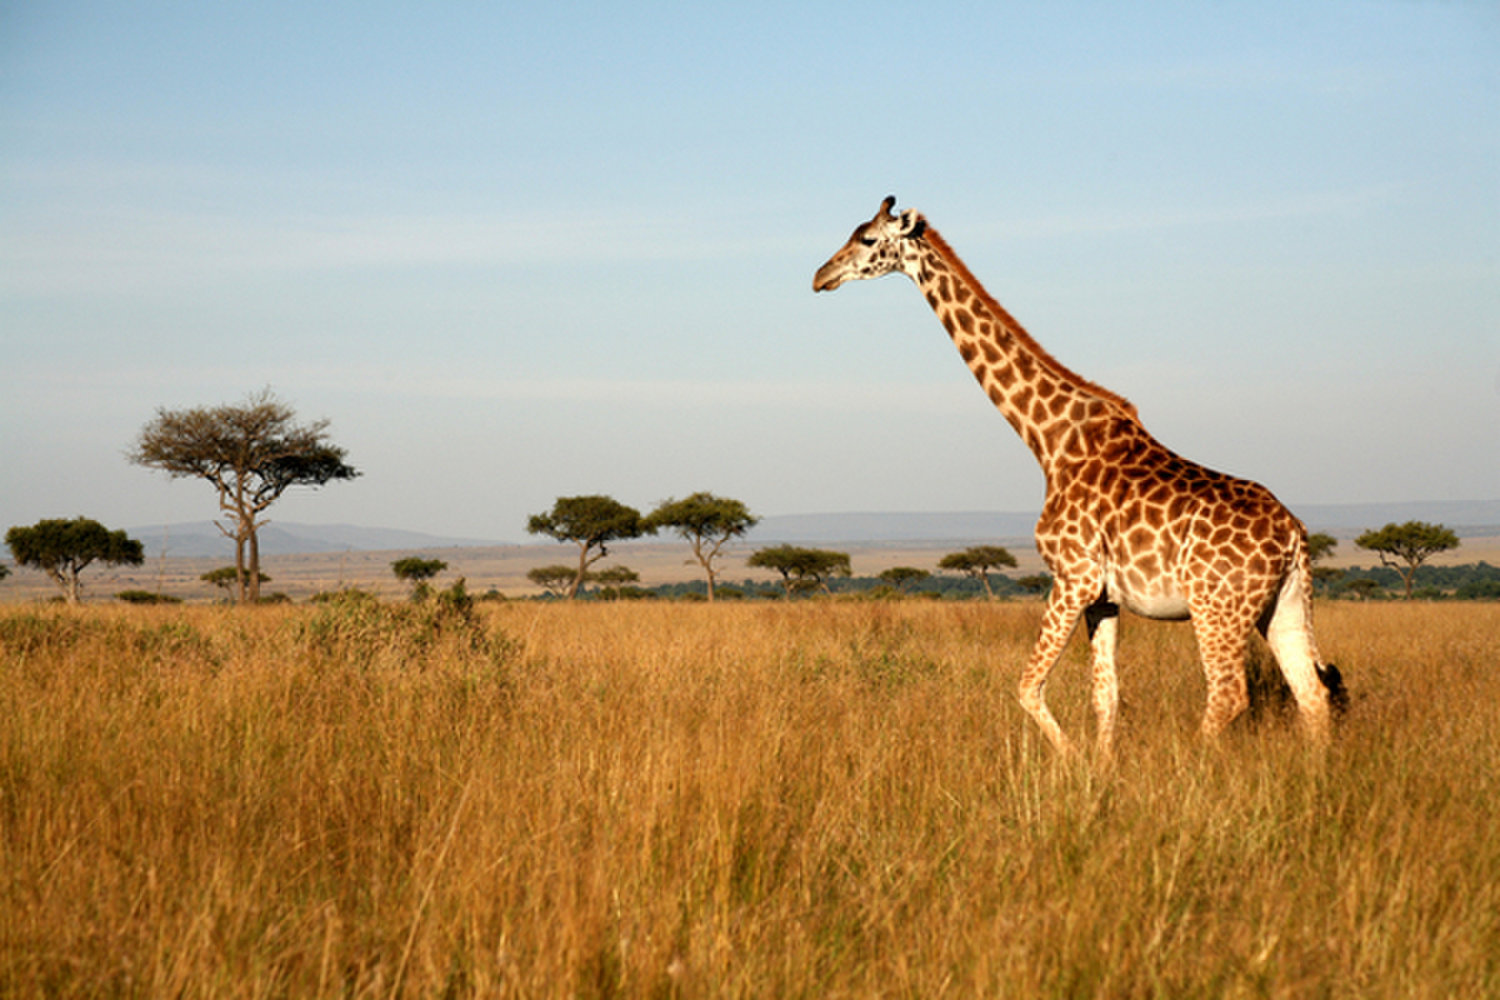
\includegraphics[width=0.7\linewidth]{giraffe1}
		\end{subfigure}%
		\begin{subfigure}{0.2\linewidth}
			\begin{equation*}
				\qquad \mapsto \qquad
			\end{equation*}
		\end{subfigure}%
		\begin{subfigure}{0.4\linewidth}
			\centering
			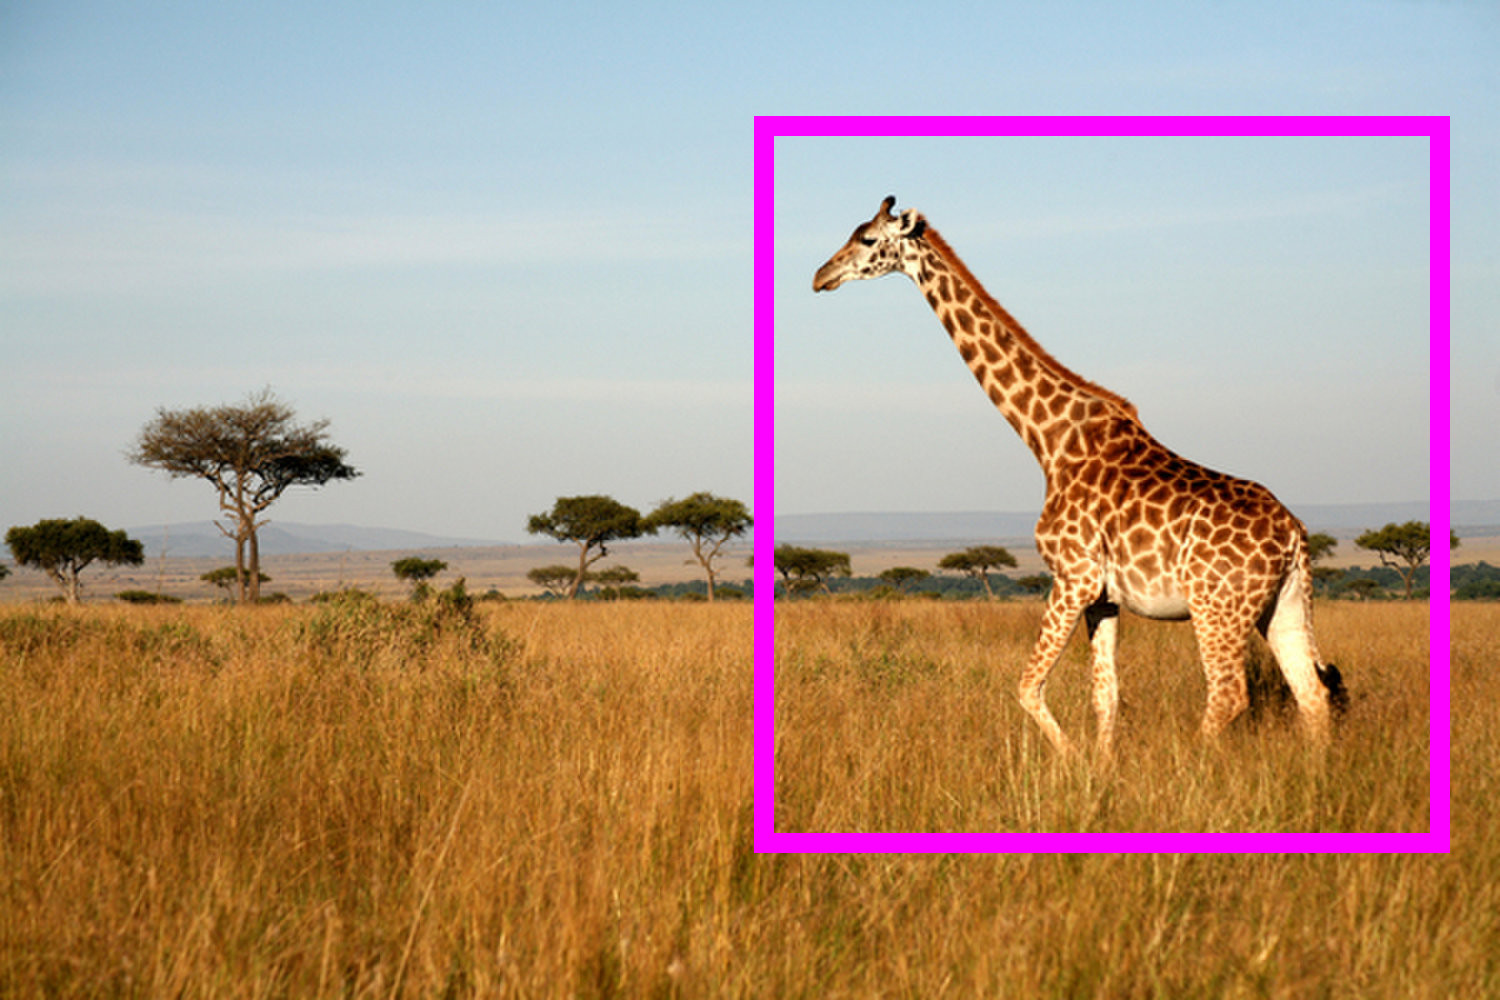
\includegraphics[width=0.7\linewidth]{giraffe1_detected}
		\end{subfigure}
	\end{figure}}
	\onslide<4->{
	Robot trajectories:
	\begin{figure}
		\begin{subfigure}{0.4\linewidth}
			\centering
			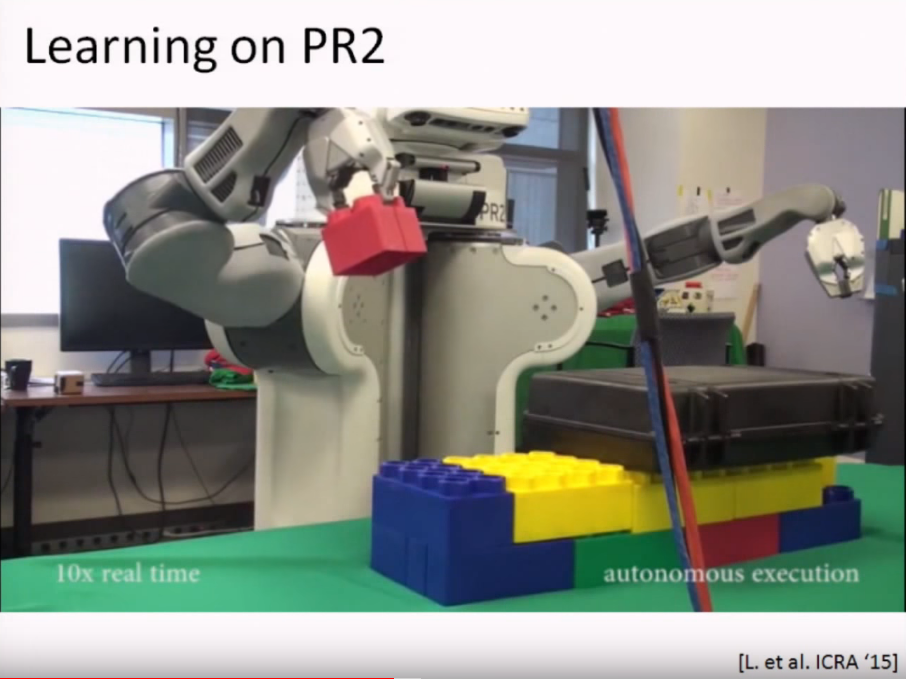
\includegraphics[width=0.7\linewidth]{robot1_f1}
		\end{subfigure}%
		\begin{subfigure}{0.2\linewidth}
			\begin{equation*}
				\qquad \mapsto \qquad
			\end{equation*}
		\end{subfigure}%
		\begin{subfigure}{0.4\linewidth}
			\centering
			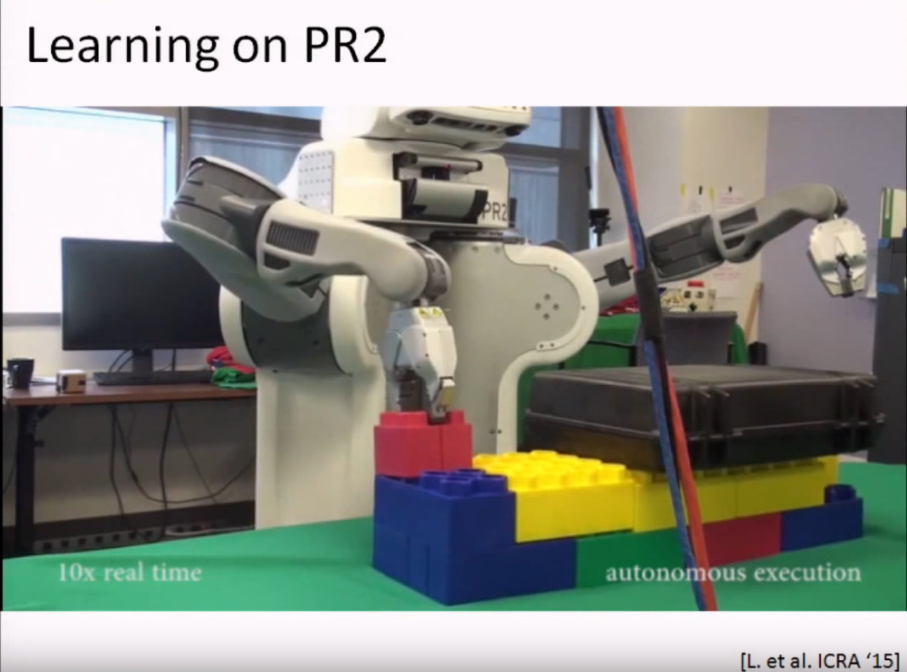
\includegraphics[width=0.7\linewidth]{robot1_f2}
		\end{subfigure}
	\end{figure}}
	
\end{frame}

\begin{frame}{Training neural networks}
		\only<1>{\begin{figure}
		\centering
		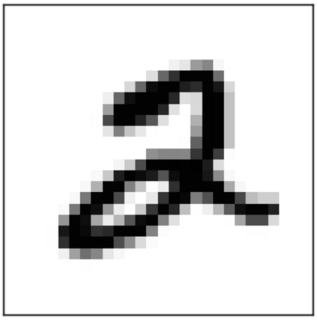
\includegraphics[scale=0.6]{backpropagation_1}
	\end{figure}}
	\only<2>{\begin{figure}
		\centering
		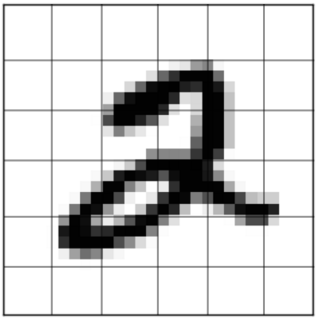
\includegraphics[scale=0.6]{backpropagation_2}
	\end{figure}}
	\only<3>{\begin{figure}
		\centering
		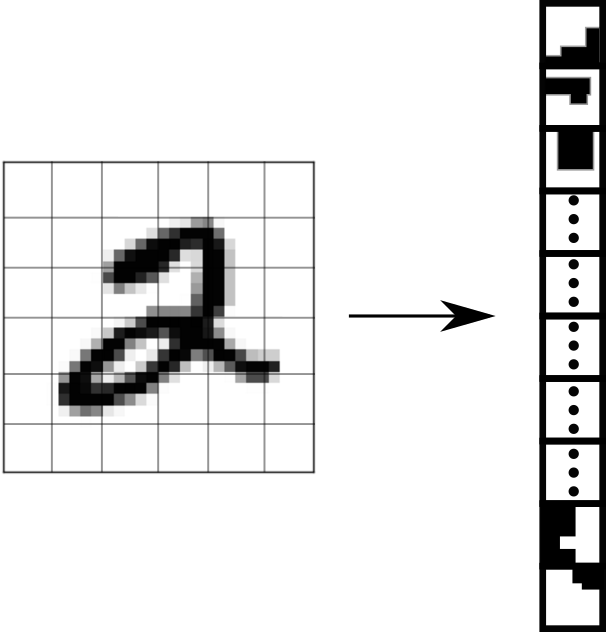
\includegraphics[scale=0.6]{backpropagation_3}
	\end{figure}}
	\only<4>{\begin{figure}
		\centering
		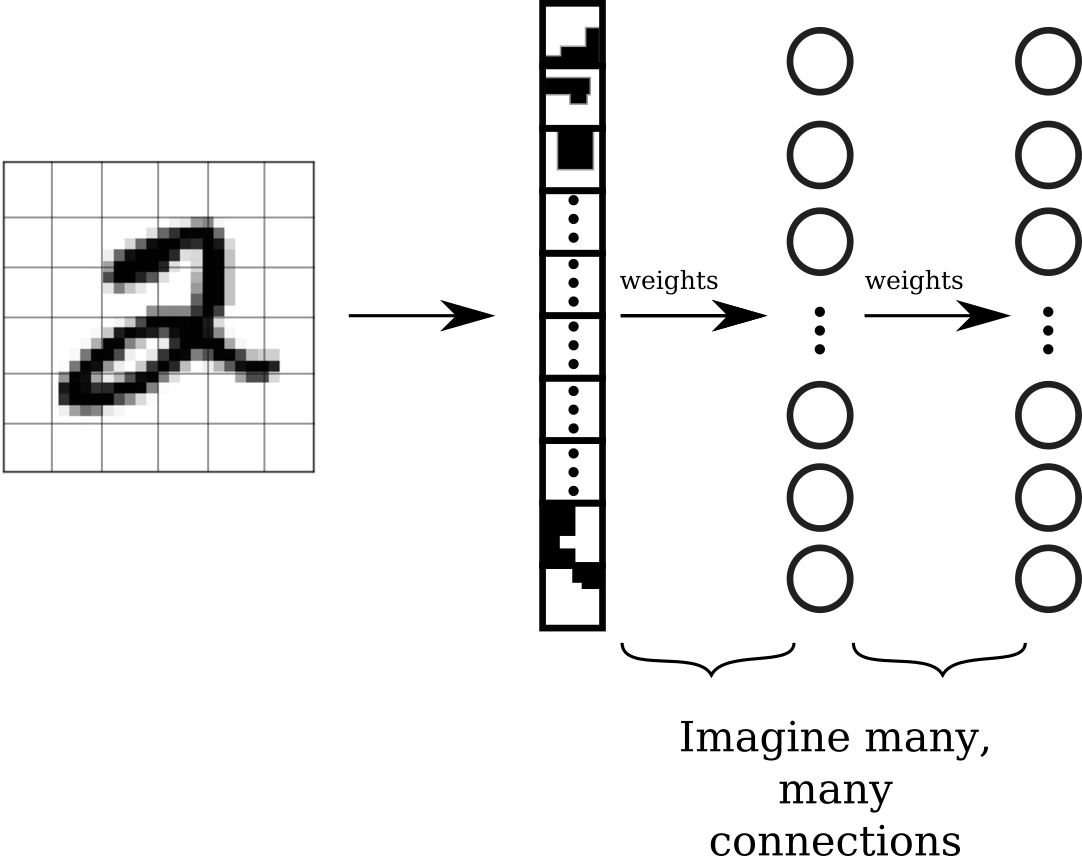
\includegraphics[scale=0.6]{backpropagation_4}
	\end{figure}}
	\only<5>{\begin{figure}
		\centering
		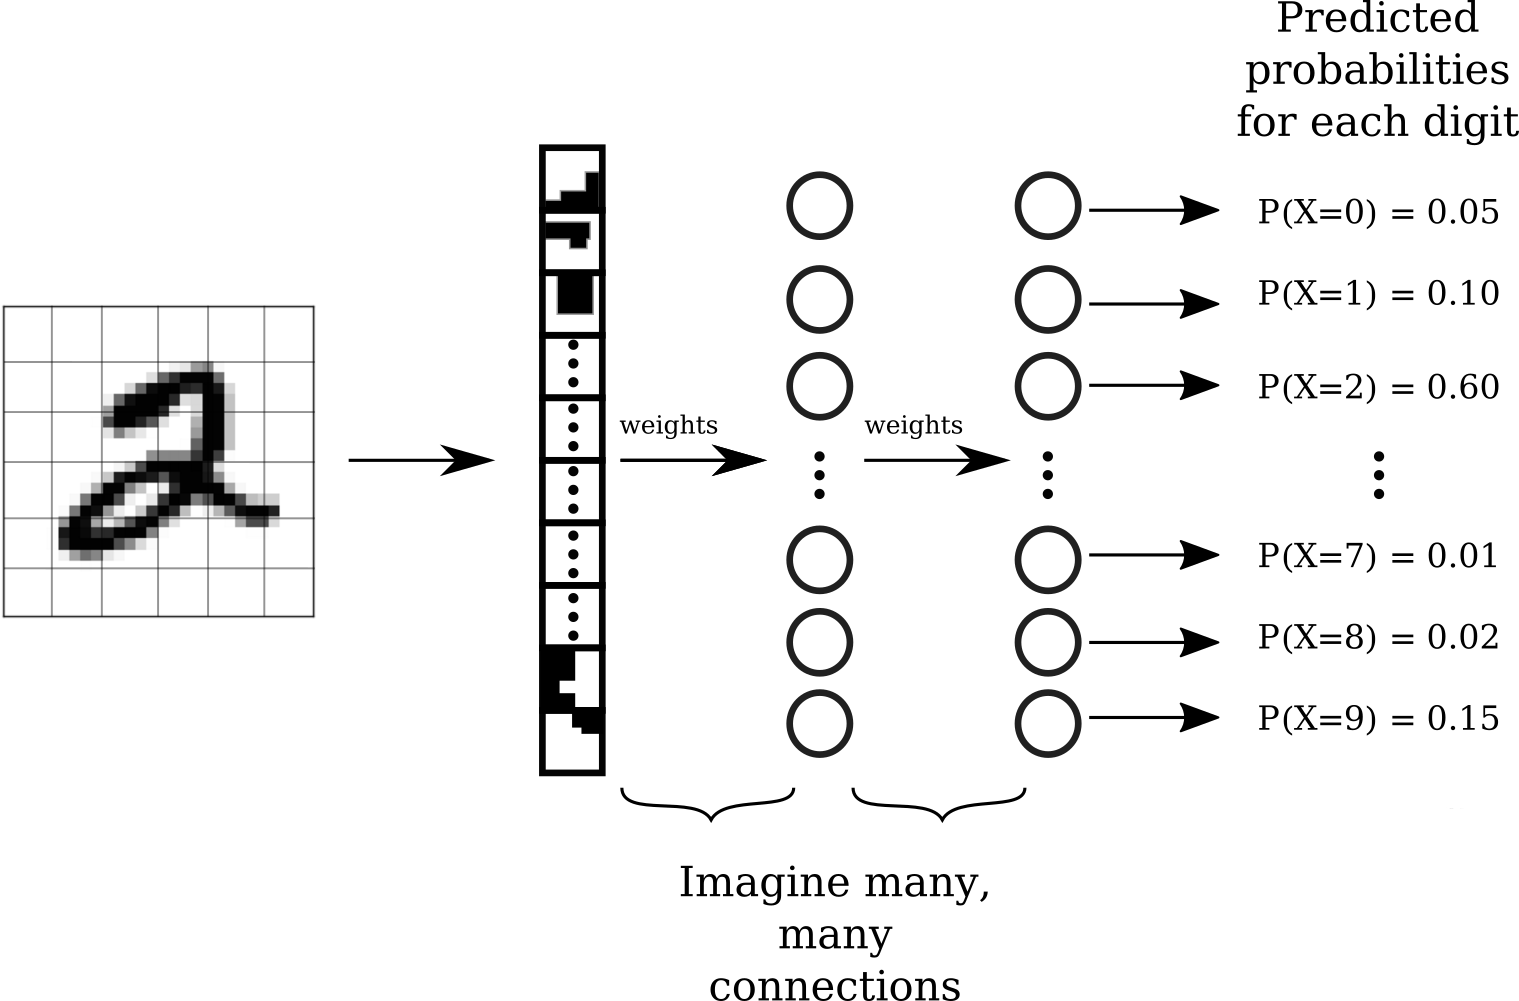
\includegraphics[scale=0.6]{backpropagation_5}
	\end{figure}}
	\only<6>{\begin{figure}
		\centering
		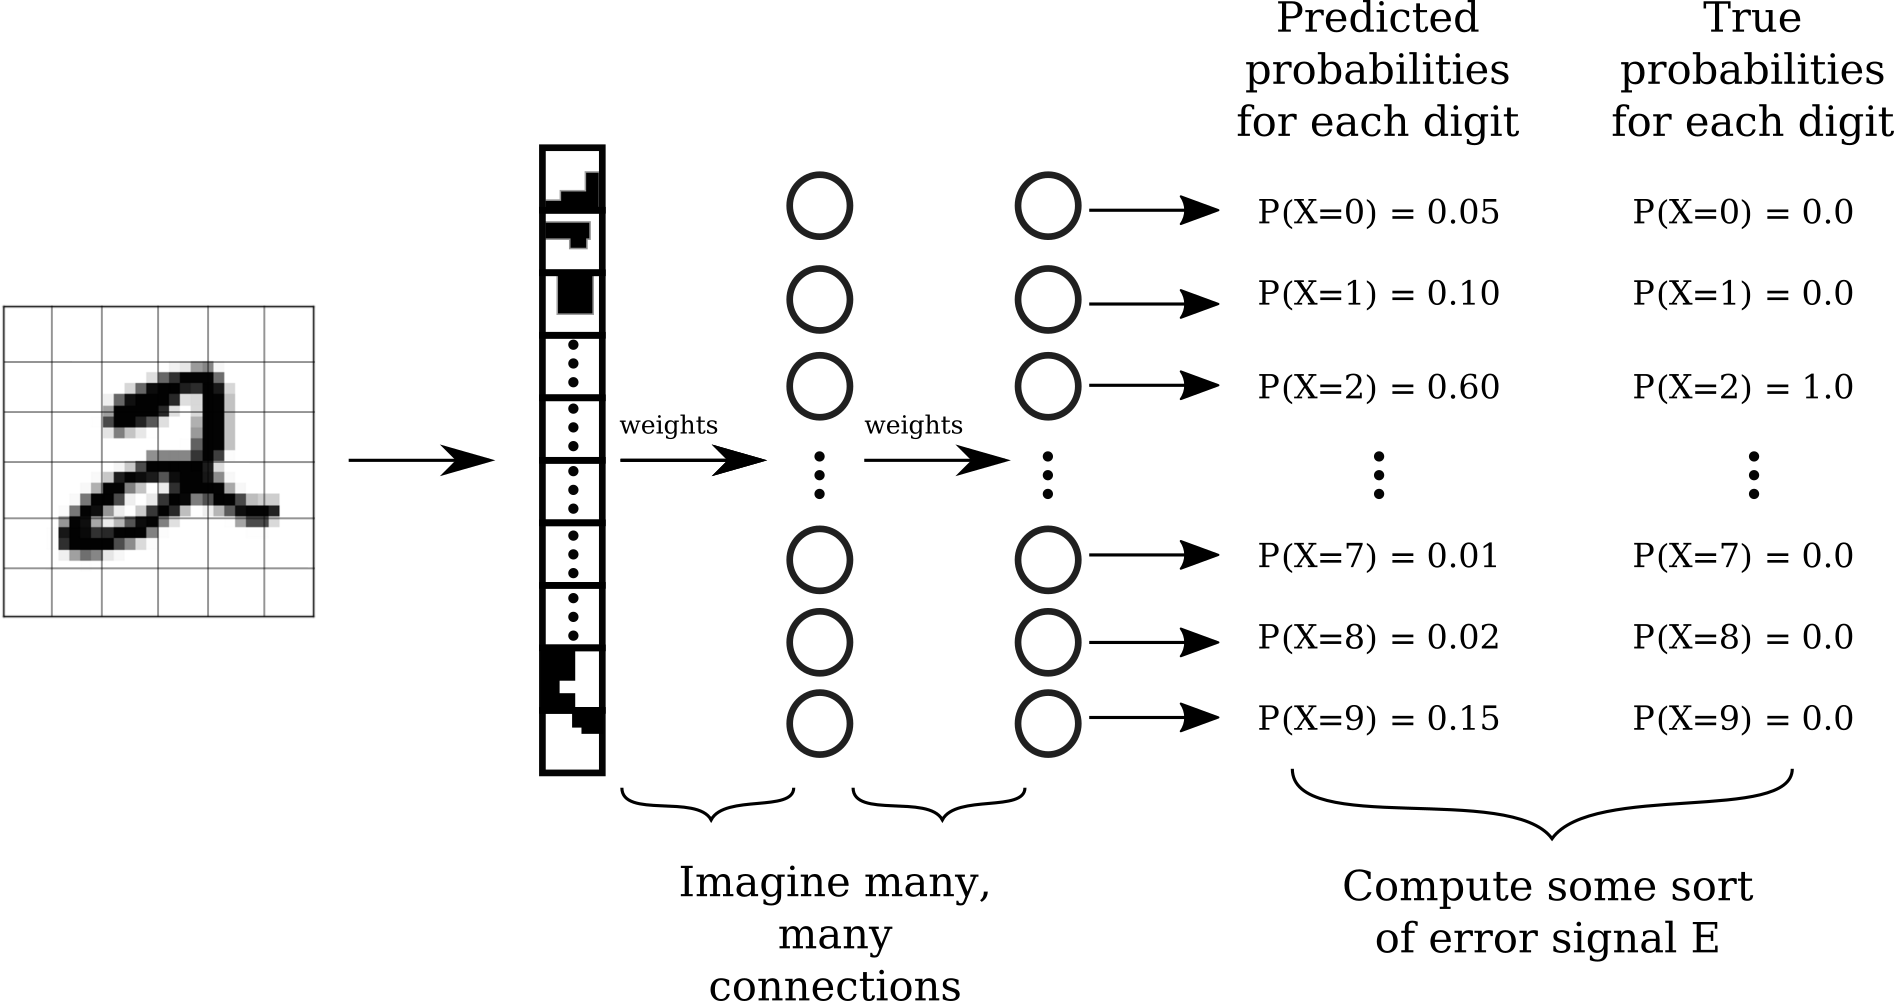
\includegraphics[scale=0.6]{backpropagation_6}
	\end{figure}}
	\only<7>{\begin{figure}
		\centering
		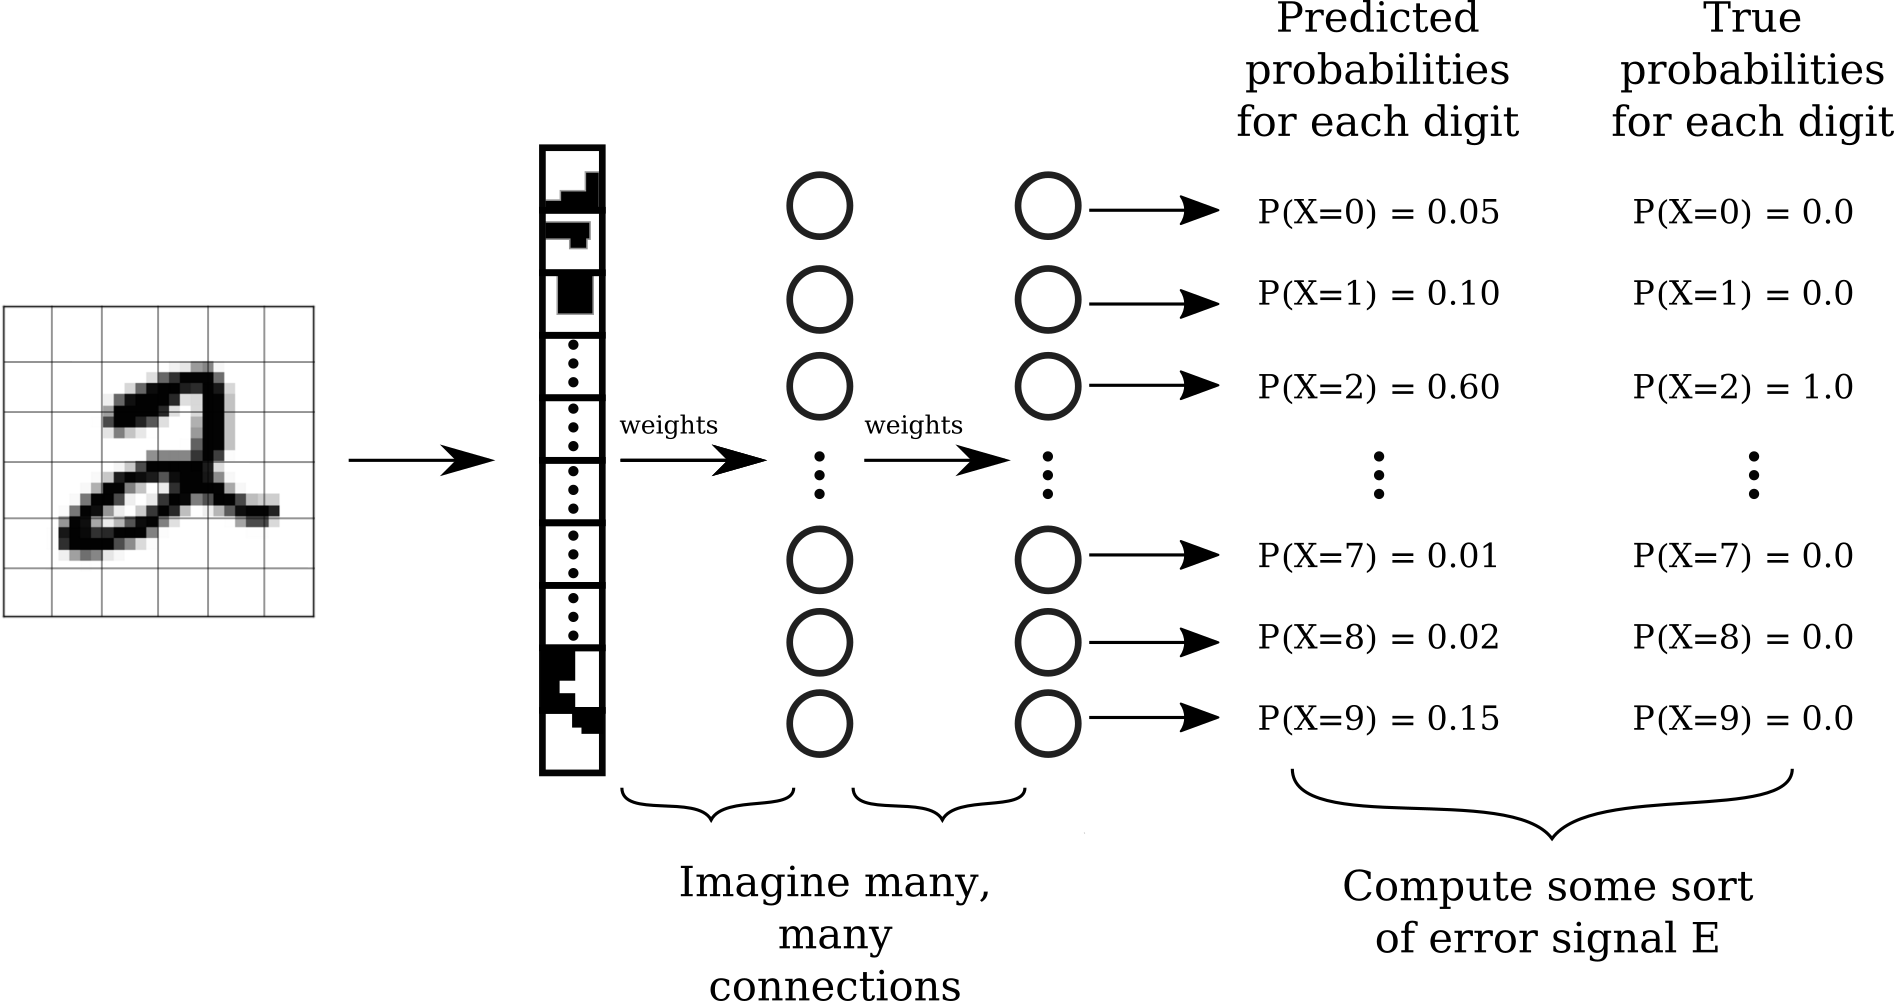
\includegraphics[scale=0.6]{backpropagation_7}
	\end{figure}}
	\only<8>{\begin{figure}
		\centering
		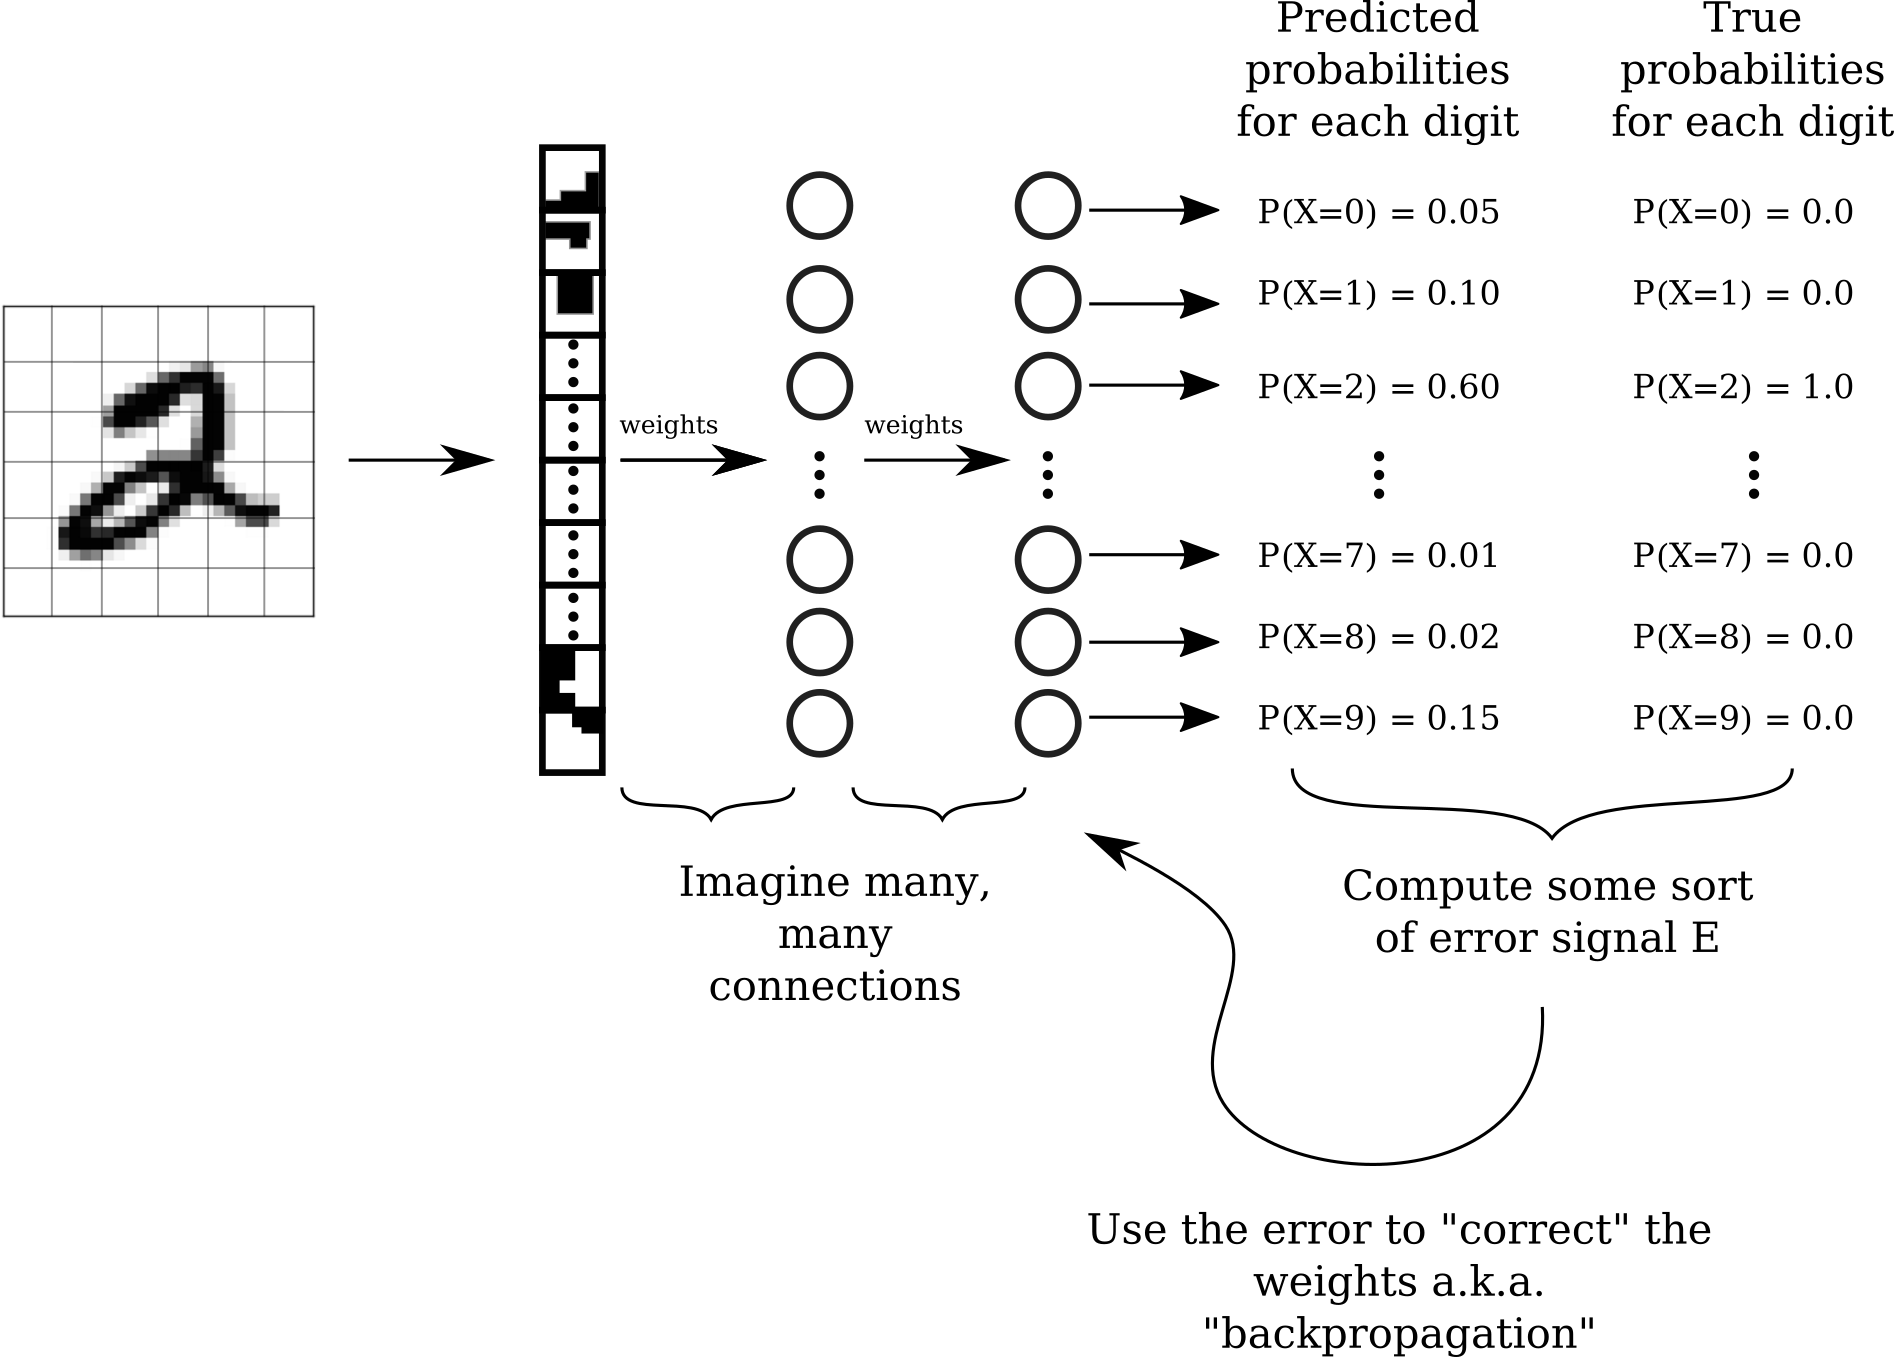
\includegraphics[scale=0.6]{backpropagation_8}
	\end{figure}}
\end{frame}

\begin{frame}{Training neural networks}
	\begin{figure}
		\centering
		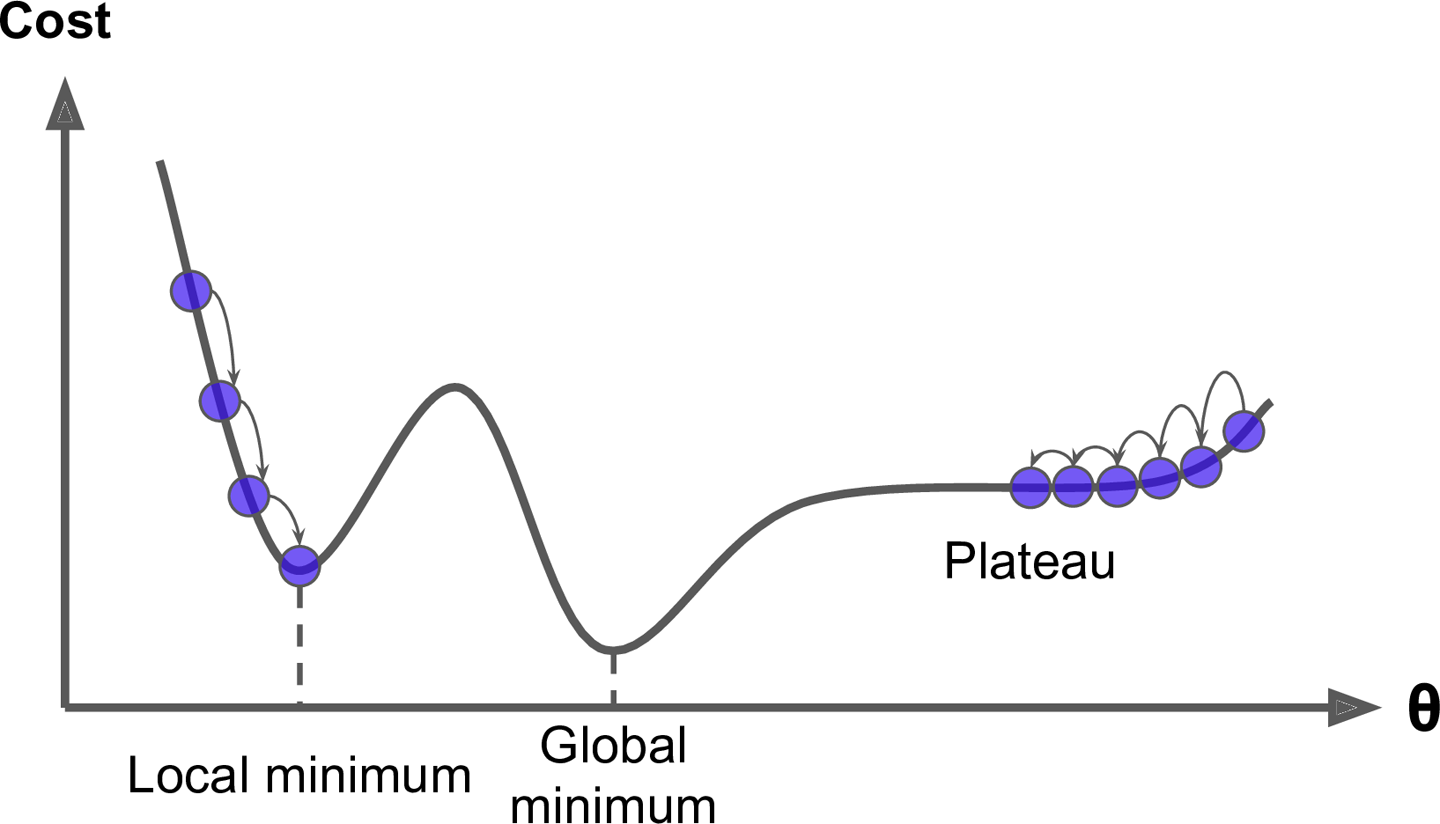
\includegraphics[scale=0.5]{gradient_descent}
	\end{figure}
	The \alert{backpropagation} algorithm is based on \alert{gradient descent}\onslide<2->{, i.e. the parameters are updated based on their current value and on their "influence" on the error.}
	\onslide<3->{
	\begin{equation*}
		\theta_{t+1} = \theta_t - \eta \frac{\partial E}{\partial \theta_t} \,,
	\end{equation*}
	\small{where $\eta$ is the \alert{learning rate}.}}
\end{frame}

\begin{frame}{How to deep learn? The naive approach}
	\onslide<2->{
	\begin{figure}
		\centering
		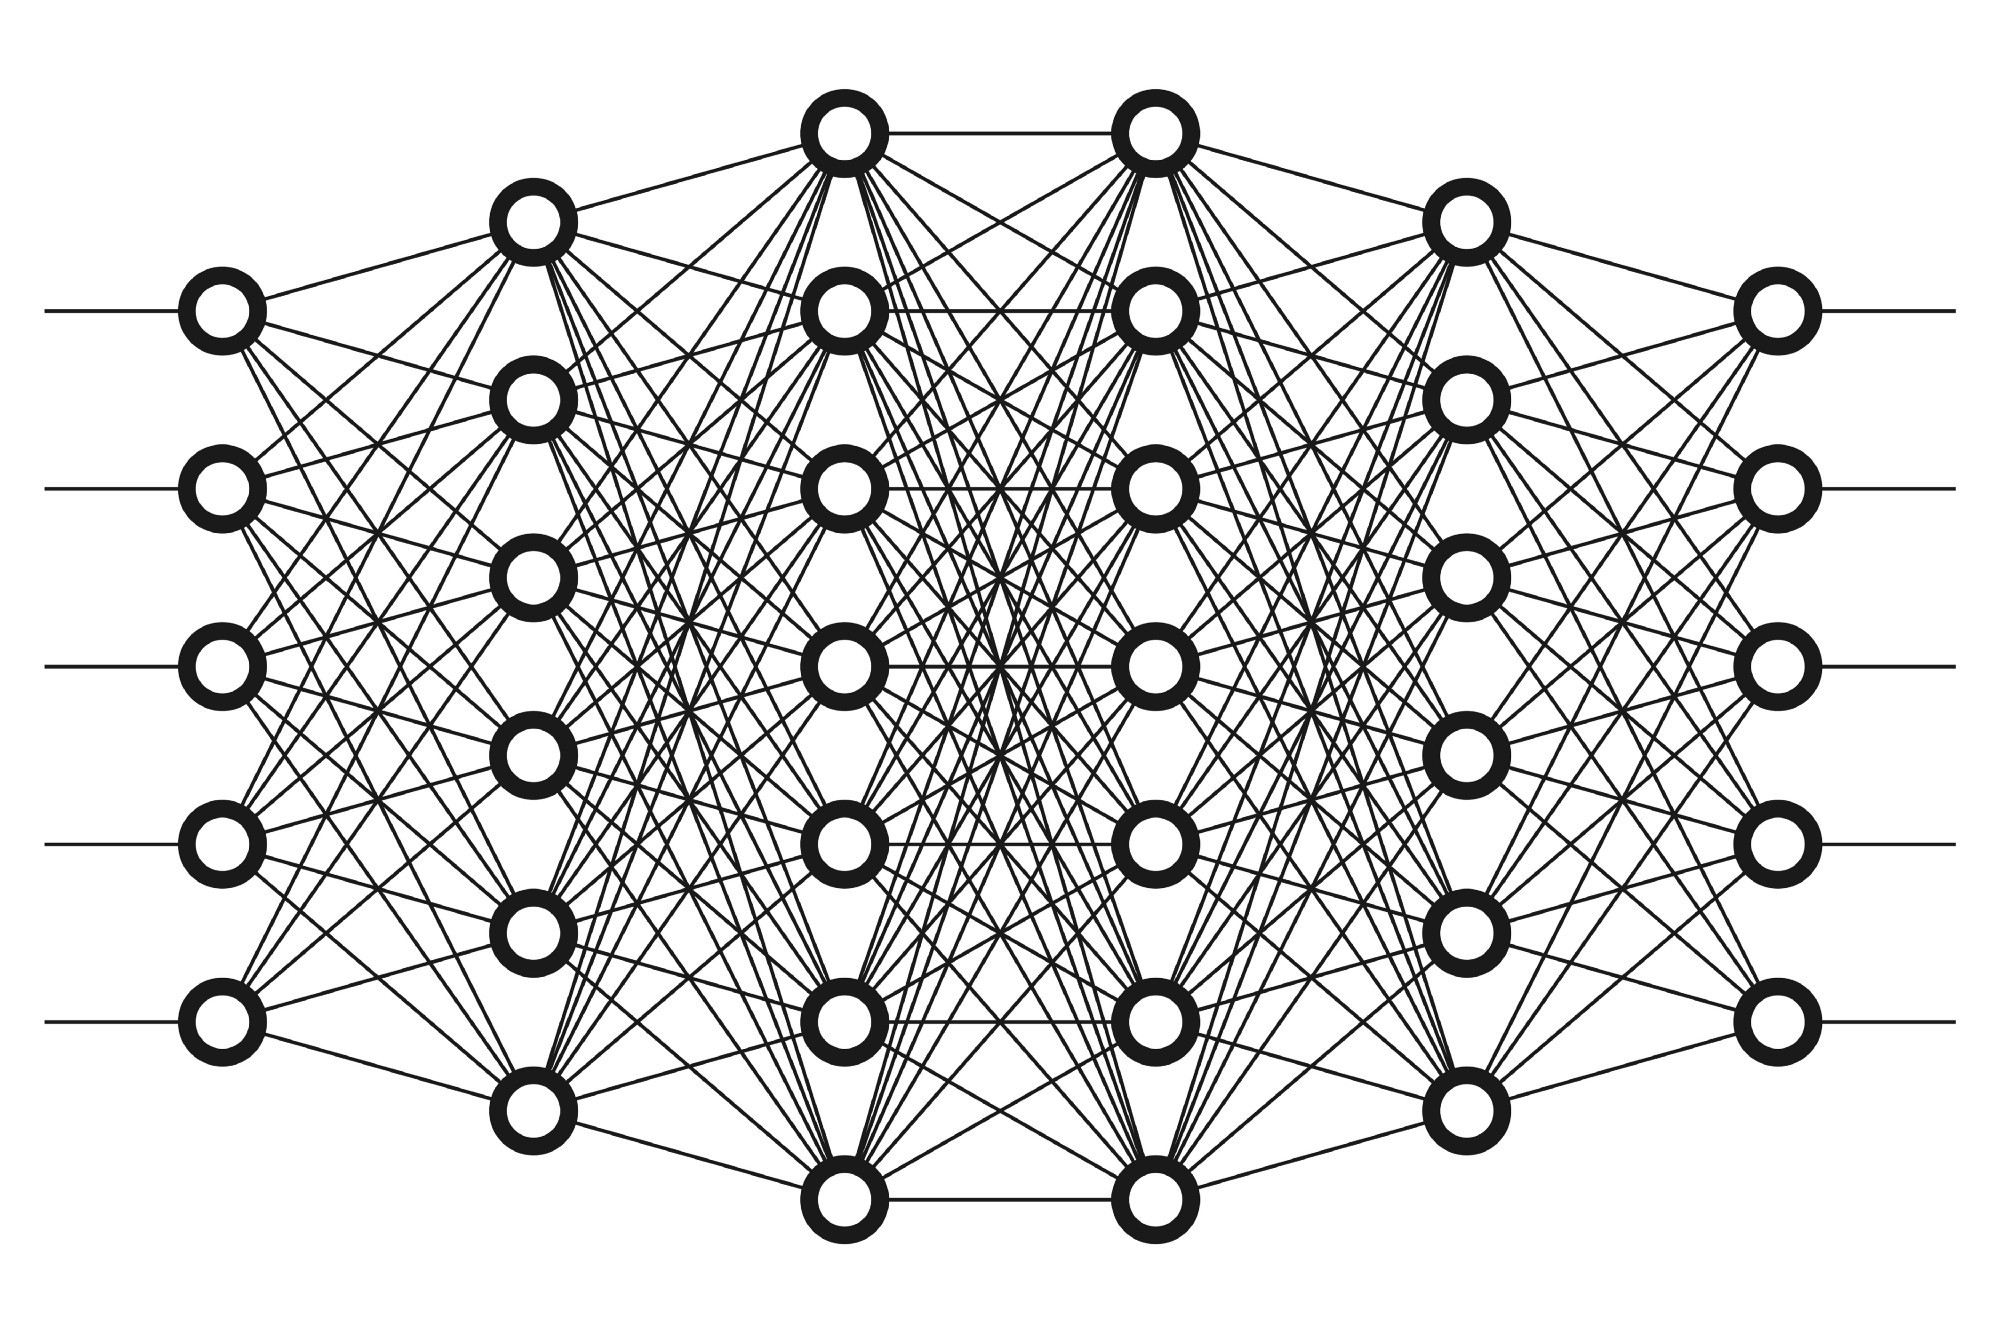
\includegraphics[width=0.8\textwidth]{deeplearningnaive}
	\end{figure}}
	\onslide<3->{
	Just stacking more simple layers will result in a \alert{inefficient} and \alert{difficult to train} network.}
\end{frame}

\begin{frame}{Some of the new things}
	\begin{figure}
		\begin{subfigure}{0.3\textwidth}
			\centering
			\onslide<2->{
			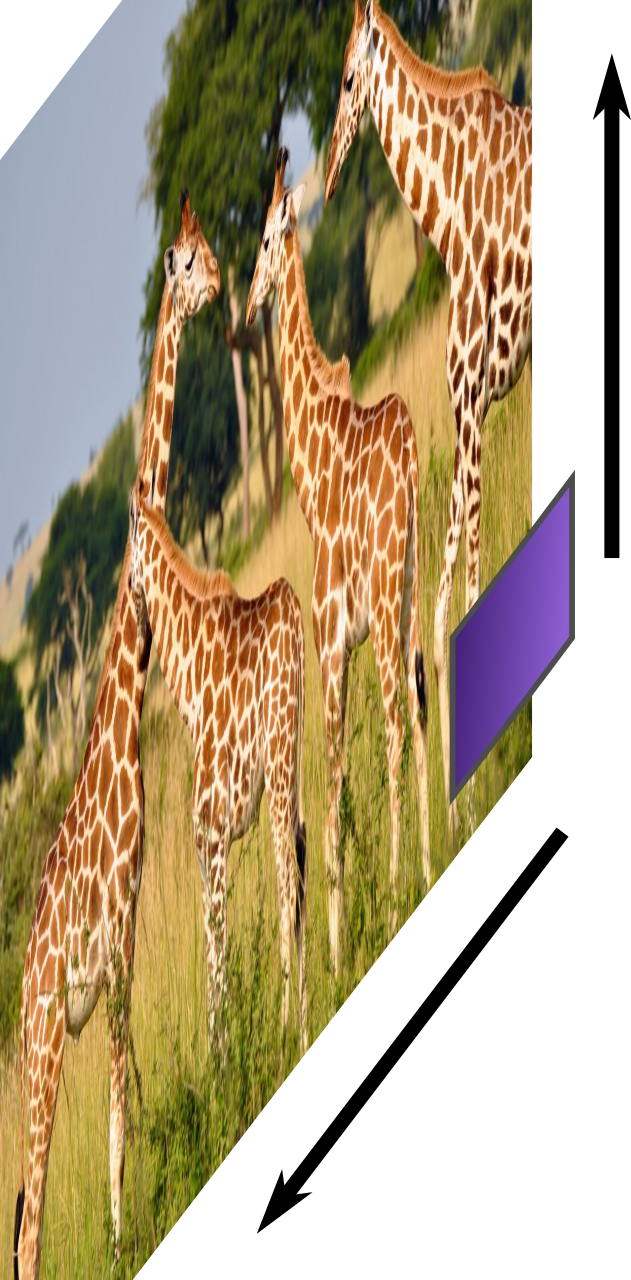
\includegraphics[width=0.7\linewidth]{convolutional_neuron}
			Convolutional neuron}
		\end{subfigure}%
		\begin{subfigure}{0.3\textwidth}
			\centering
			\onslide<3->{
			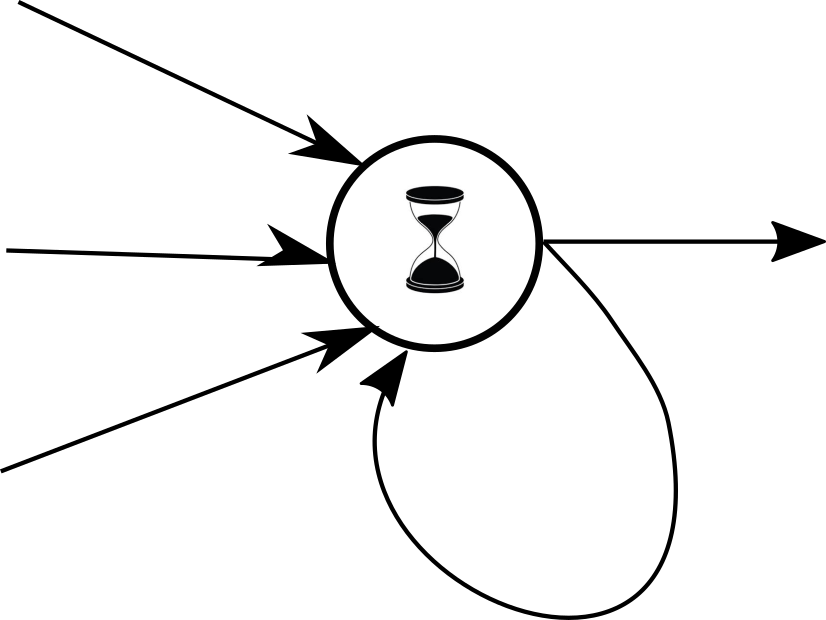
\includegraphics[width=\linewidth]{temporal_neuron}
			Memory cell neuron}
		\end{subfigure}%
		\begin{subfigure}{0.4\textwidth}
			\centering
			\onslide<4->{
			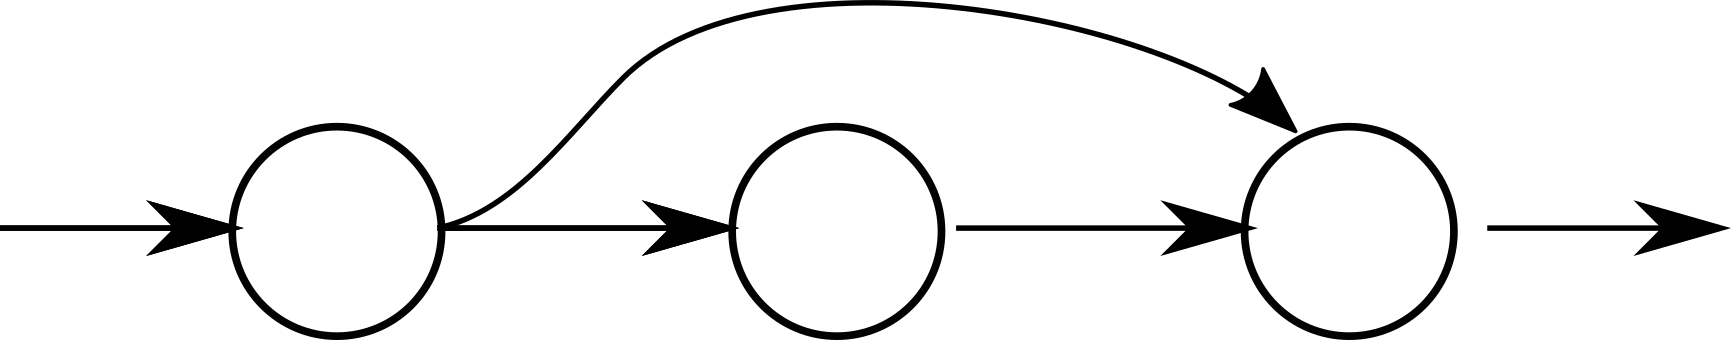
\includegraphics[width=\linewidth]{skip_neuron}
			Neuron with skip connections}
		\end{subfigure}
	\end{figure}
	\onslide<5->{
	\alert{Any} kind of \alert{differentiable} function can be a neuron!}
\end{frame}

\begin{frame}{Deep learning networks as computational graphs}
	\only<2>{\begin{figure}
		\centering
		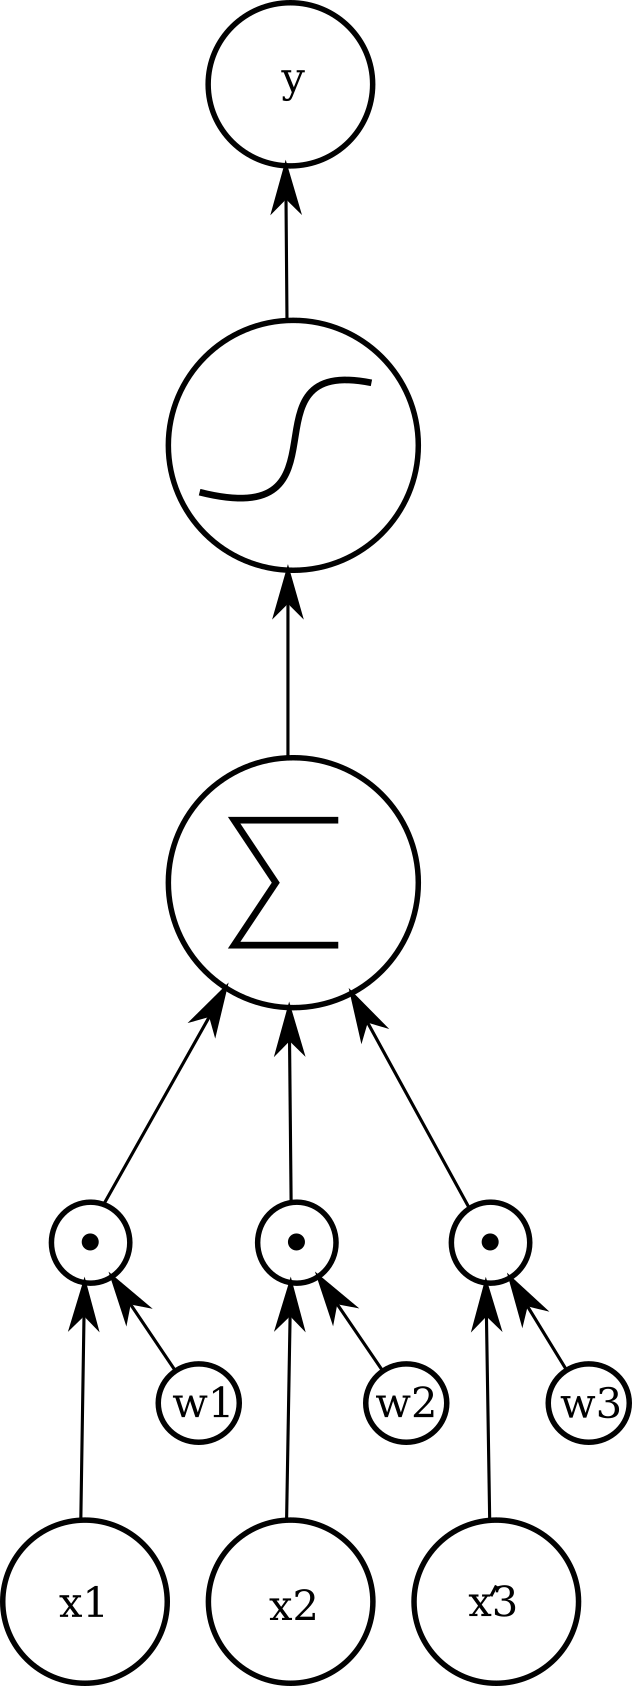
\includegraphics[scale=0.4]{flowgraph1}
	\end{figure}}
	\only<3>{\begin{figure}
		\centering
		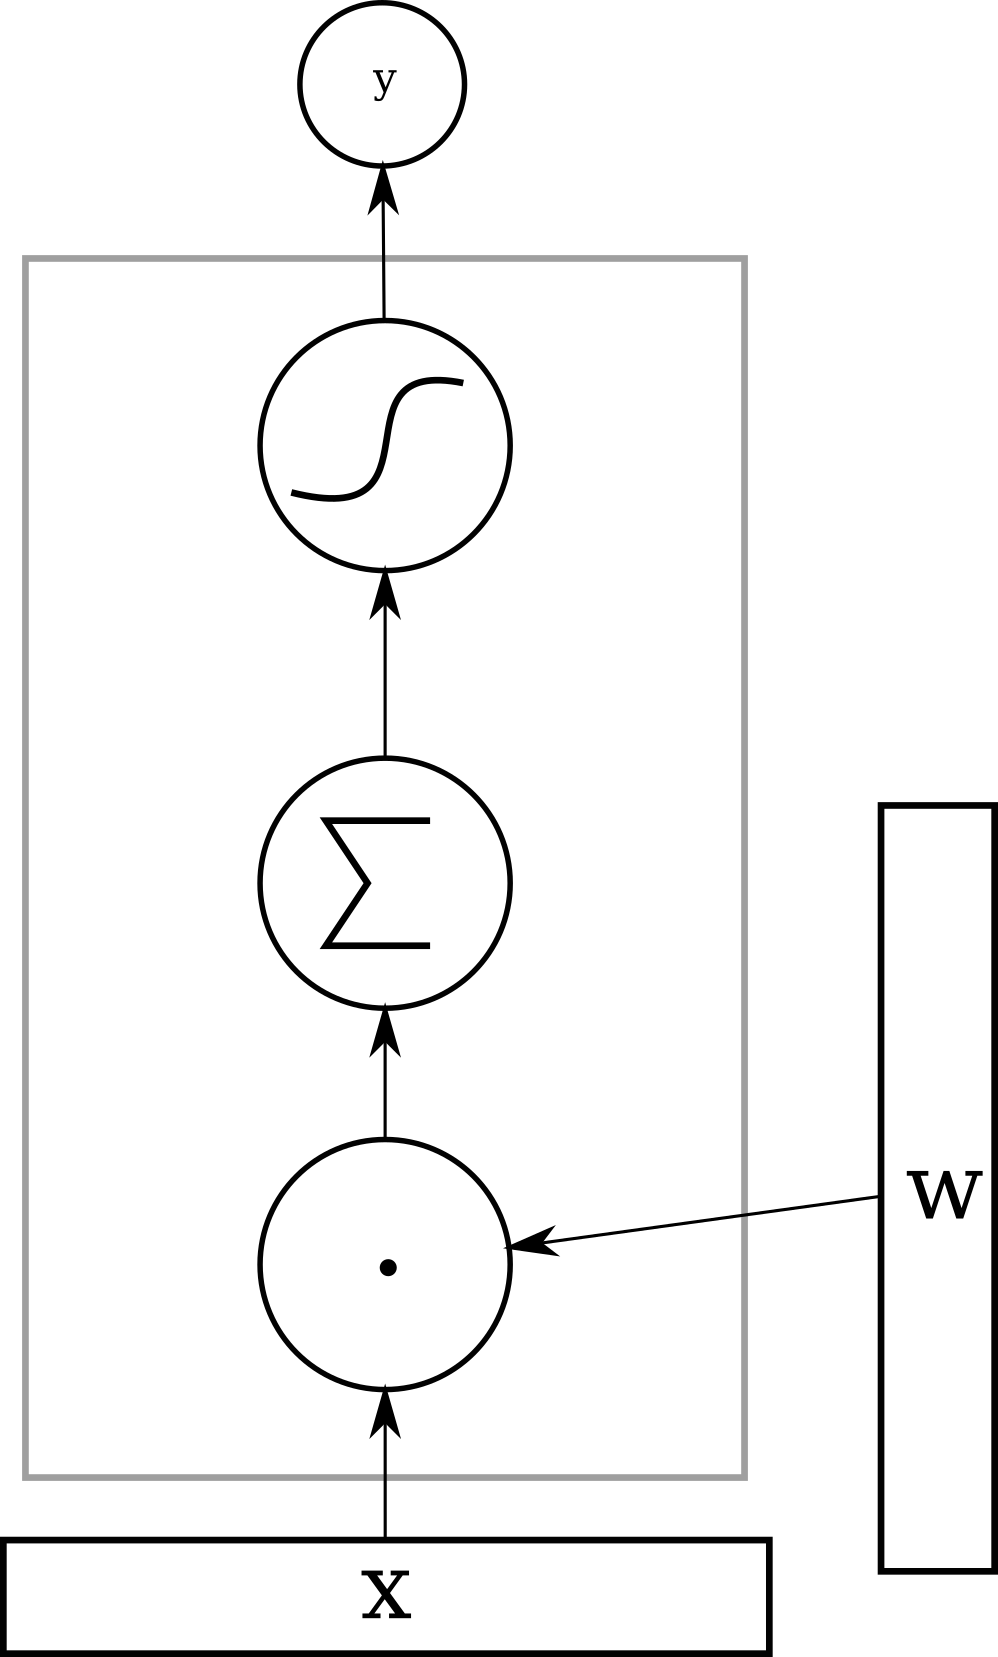
\includegraphics[scale=0.4]{flowgraph2}
	\end{figure}}
	\only<4>{\begin{figure}
		\centering
		
\includegraphics[scale=0.4]{flowgraph3}
	\end{figure}}
	\only<5>{\begin{figure}
		\centering
		
\includegraphics[scale=0.35]{flowgraph4}
	\end{figure}}
	\only<6>{\begin{figure}
		\centering
		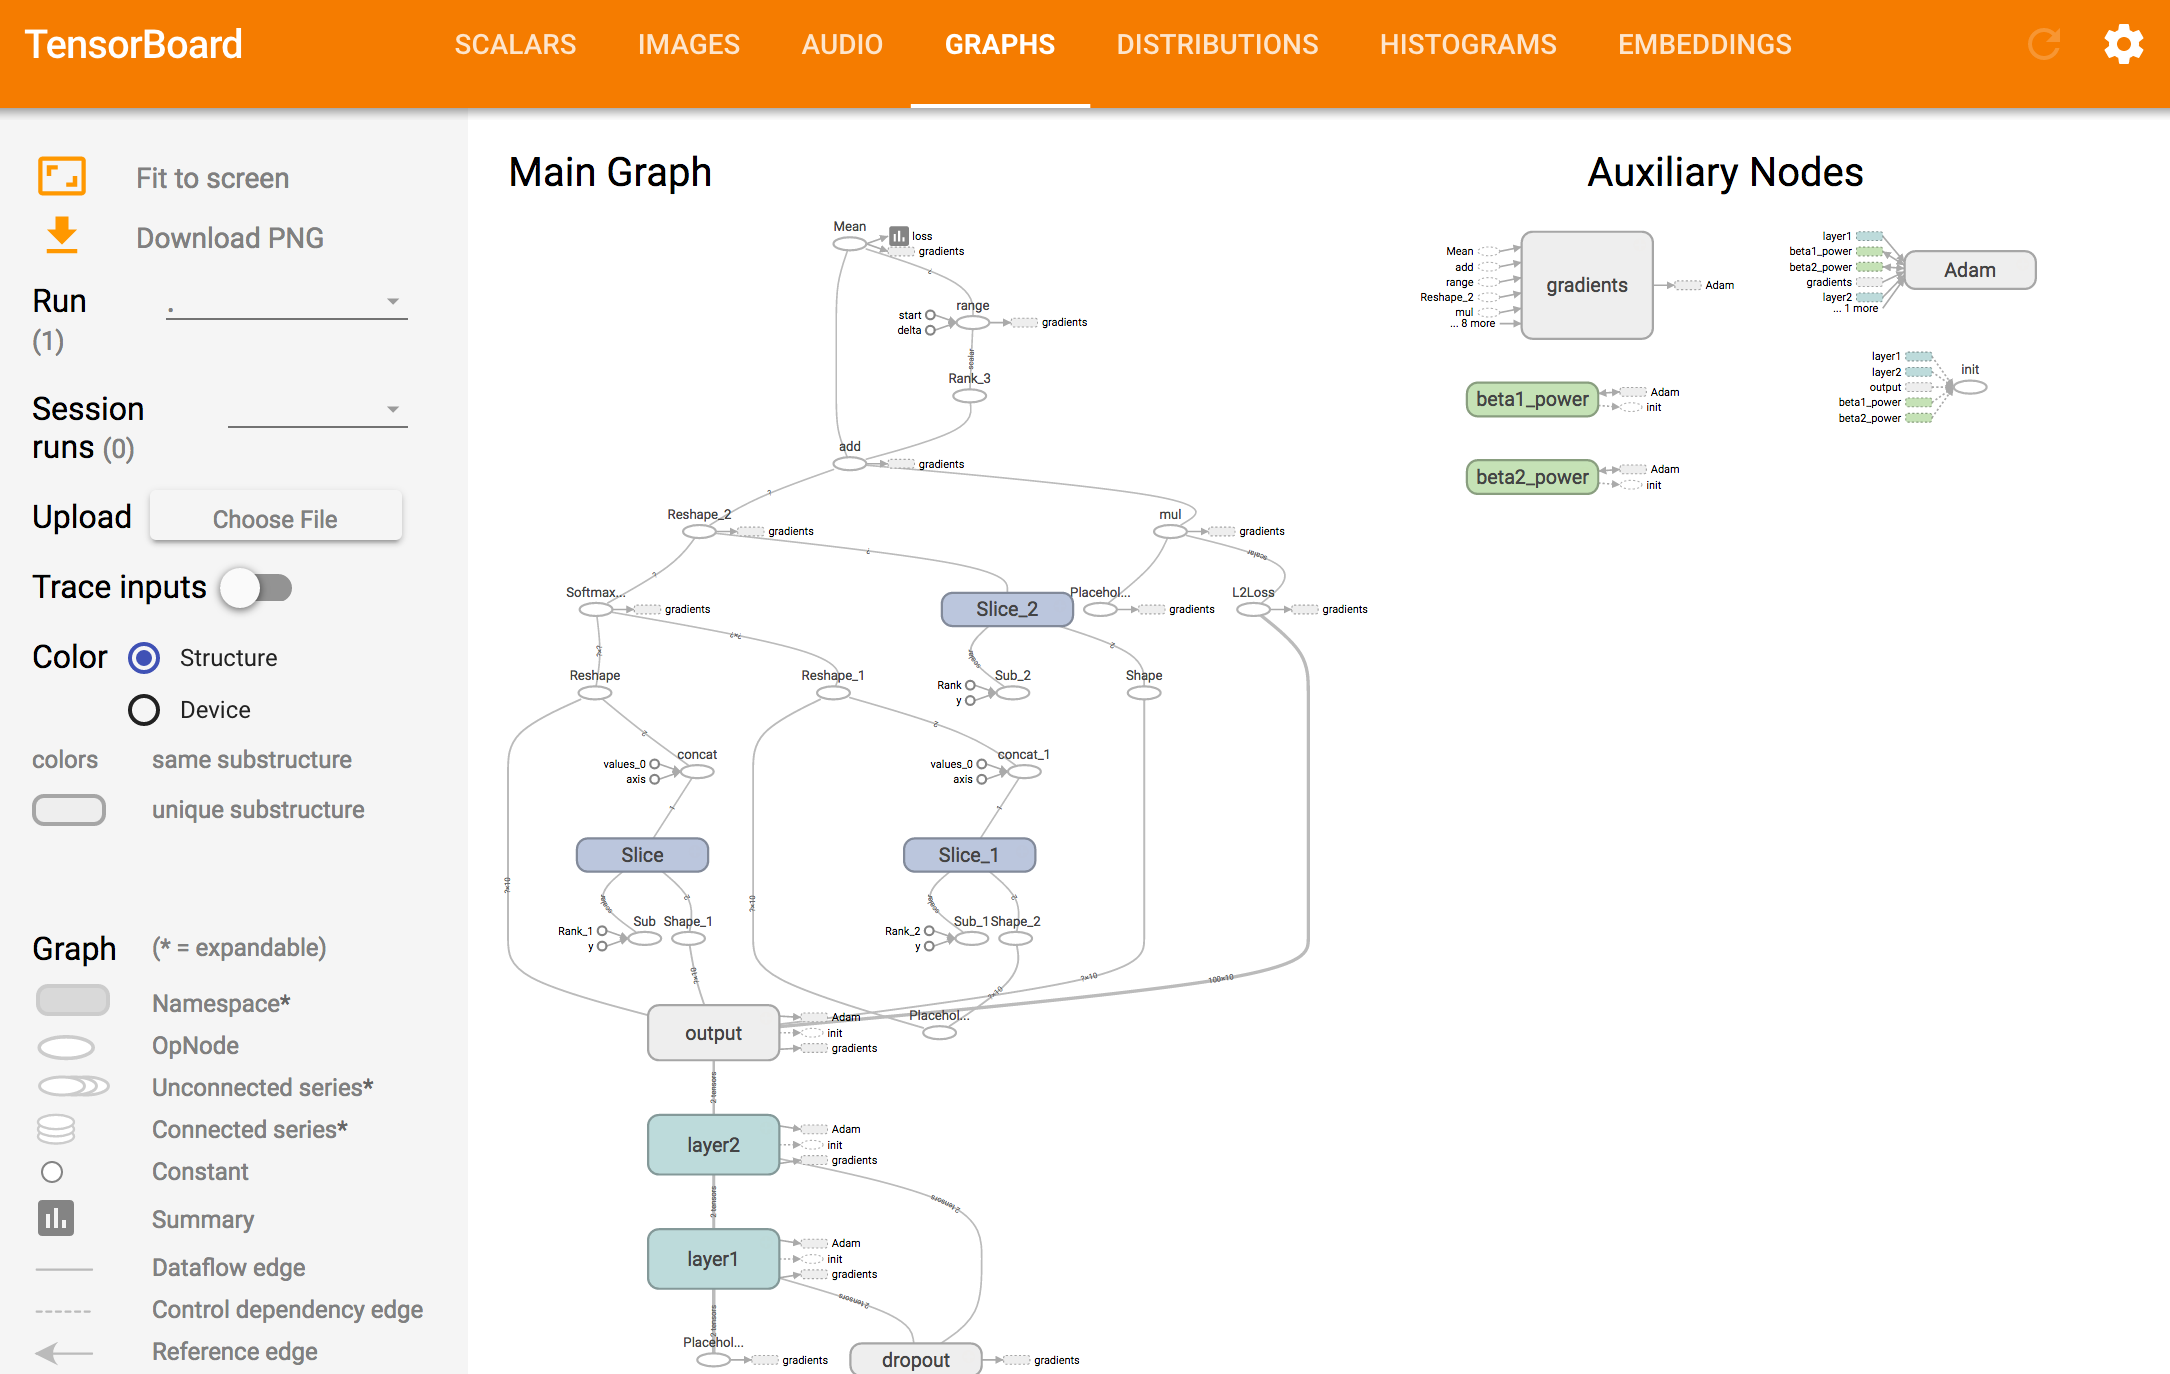
\includegraphics[width=\linewidth]{tensorboard}
	\end{figure}}
\end{frame}

\begin{frame}{The convolution operation}
	\begin{figure}
		\centering
		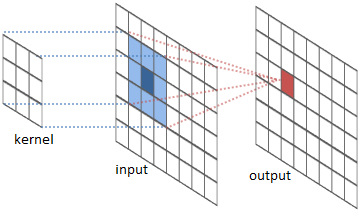
\includegraphics[scale=1.0]{convolution_operation}		
	\end{figure}
	The neuron in this case is actually the \alert{kernel}. Each value in the kernel represents a \alert{weight}. Each weight is \alert{learned}. 
\end{frame}

\begin{frame}{A classification network}
	\begin{figure}
		\centering
		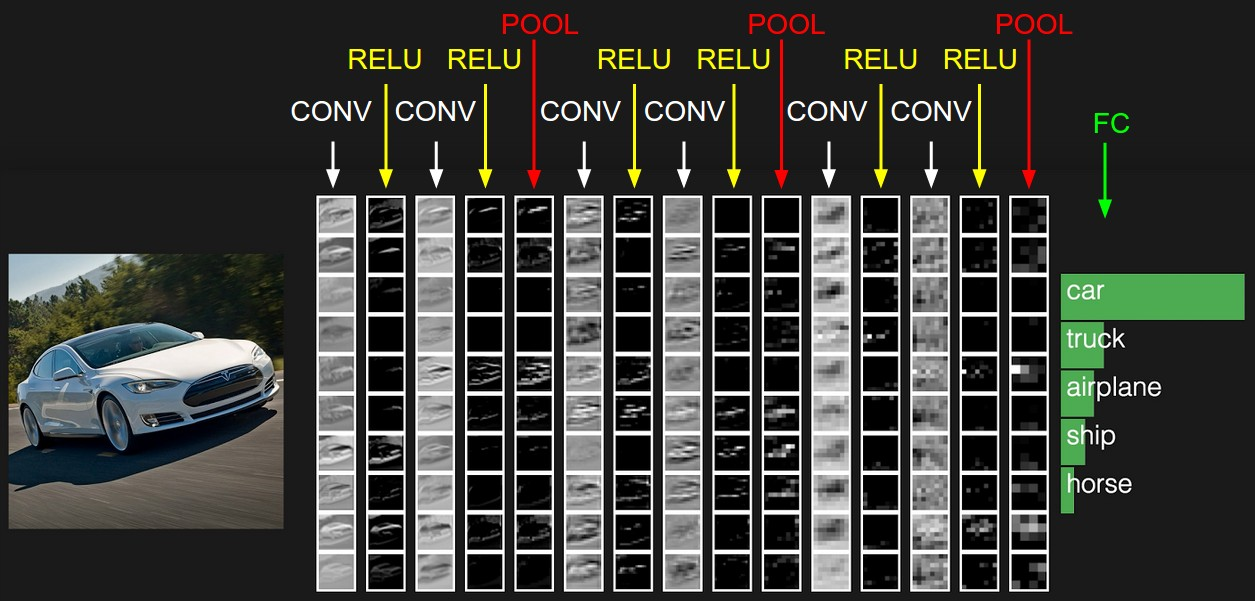
\includegraphics[width=\linewidth]{classification-network2}
	\end{figure}
\end{frame}

\begin{frame}{Another classification network}
	\begin{figure}
		\centering
		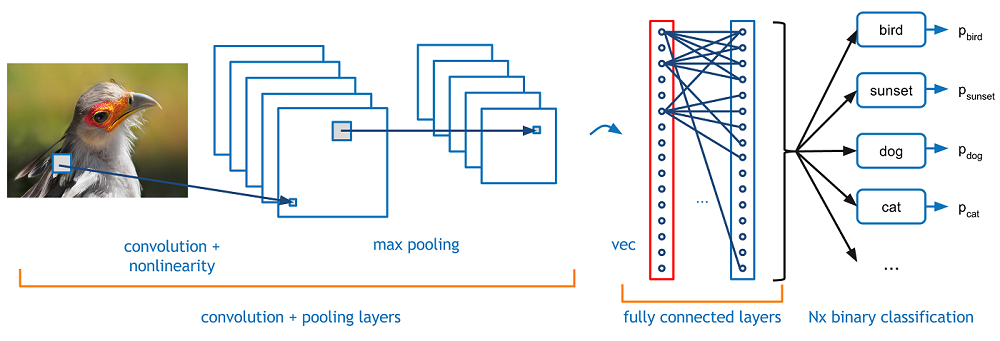
\includegraphics[width=\linewidth]{deeplearning-intro-ml}
		\caption{A deep classification network using convolutional neurons.}
	\end{figure}
	\onslide<2->{
	Super powers of deep learning:}
	\begin{itemize}
		\item<3-> general framework
		\item<4-> efficient structure
		\item<5-> well performing \onslide<6->{given the right circumstances}
	\end{itemize}
\end{frame}


\section{Do they really use it?}

\begin{frame}{Applications of deep learning}
	\onslide<2->{
	Image processing:}
	\begin{itemize}
		\item<3-> image classification
		\item<4-> object detection
		\item<5-> automatic image captioning
		\item<6-> image generation
	\end{itemize}
\end{frame}
\begin{frame}{Applications of deep learning}
	\onslide<1->{
	Control related (reinforcement learning):}
	\begin{itemize}
		\item<2-> game playing
		\item<3-> robot manipulation
	\end{itemize}
\end{frame}
\begin{frame}{Applications of deep learning}
	Medicine, biology and chemistry:
	\begin{itemize}
		\item<2-> tumor identification in medical imaging
		\item<3-> genome mutation identification (DeepVariant)
		\item<4-> automatic chemical design
	\end{itemize}

    \small{More interesting applications can be found \href{http://www.yaronhadad.com/deep-learning-most-amazing-applications/ }{\textbf{here}} and \href{https://github.com/hussius/deeplearning-biology}{\textbf{here}}.}
\end{frame}
\begin{frame}{Let's view some nice examples}
    \begin{itemize}
        \item \href{https://www.youtube.com/watch?v=VOC3huqHrss}{\textbf{YOLO object detection}}
		\item Pix2Pix \href{https://affinelayer.com/pixsrv/}{\textbf{demo}} and \href{https://twitter.com/search?vertical=default&q=edges2cats&src=typd}{\textbf{Twitter hashtag}}
		\item \href{https://www.youtube.com/watch?v=3AIpPlzM_qs}{\textbf{Pix2PixHD}} 
		\item \href{https://www.youtube.com/watch?v=ys5nMO4Q0iY}{\textbf{Automatic image colorization}}
		\item \href{https://www.youtube.com/watch?time_continue=22&v=pW6nZXeWlGM}{\textbf{Pose estimation}}
		\item \href{https://youtu.be/V1eYniJ0Rnk?t=25s}{\textbf{Atari game playing}}
		\item \href{https://www.youtube.com/watch?v=L4KBBAwF_bE}{\textbf{Super Mario}}
		\item \href{https://youtu.be/ZhsEKTo7V04?t=18s}{\textbf{Robotic manipulation}}
    \end{itemize}
\end{frame}

\section{Deep learning and me}

\begin{frame}{Is deep learning right for you?}
You should consider deep learning if:
\begin{itemize}
	\item<2-> you have access to quite large amounts of data
    \item<3-> the problem is reasonably complex, in a high dimensional space
	\item<4-> no hard constraints or hard logic
\end{itemize}
\end{frame}

\begin{frame}{Where do I start?}
	\begin{columns}
		\begin{column}{0.5\textwidth}
			\onslide<2->{
			Frameworks and software (usually require \alert{GPUs}):}
			\begin{itemize}
				\item<3-> Tensorflow
				\item<4-> PyTorch
				\item<5-> Matlab
			\end{itemize}
		\end{column}
		\begin{column}{0.5\textwidth}
			\onslide<6->{Learning resources:}
			\begin{itemize}
				\item<7-> Stanford CS231n course (Karpathy et. al.)
				\item<8-> Deep learning book (Goodfellow)
				\item<9-> various YouTube videos
                \item<10-> For beginners: \href{https://www.reddit.com/r/machinelearning}{\textbf{/r/LearnMachineLearning}}
                \item<11-> After you grasp the concepts: \href{https://www.reddit.com/r/machinelearning}{\textbf{/r/MachineLearning}}
                \item<12-> the Twitter pages of various deep learning celebrities
				\item<13-> more at \href{https://github.com/ChristosChristofidis/awesome-deep-learning}{\textbf{this}} link
			\end{itemize}
		\end{column}
	\end{columns}
\end{frame}

\begin{frame}[standout]
	Thank you for your attention!\\
	\vspace{2cm}
	Questions?\\
	\vspace{1.5cm}
	\small{Slides can be found at \url{www.github.com/pauldragan}.}
	\\
	\small{You can also find me on Twitter \href{www.twitter.com/pauldragannow}{\textbf{@PaulDraganNow}}}
\end{frame}

\end{document}